% Options for packages loaded elsewhere
\PassOptionsToPackage{unicode}{hyperref}
\PassOptionsToPackage{hyphens}{url}
\PassOptionsToPackage{dvipsnames,svgnames,x11names}{xcolor}
%
\documentclass[
  letterpaper,
  DIV=11,
  numbers=noendperiod]{scrreprt}

\usepackage{amsmath,amssymb}
\usepackage{iftex}
\ifPDFTeX
  \usepackage[T1]{fontenc}
  \usepackage[utf8]{inputenc}
  \usepackage{textcomp} % provide euro and other symbols
\else % if luatex or xetex
  \usepackage{unicode-math}
  \defaultfontfeatures{Scale=MatchLowercase}
  \defaultfontfeatures[\rmfamily]{Ligatures=TeX,Scale=1}
\fi
\usepackage{lmodern}
\ifPDFTeX\else  
    % xetex/luatex font selection
\fi
% Use upquote if available, for straight quotes in verbatim environments
\IfFileExists{upquote.sty}{\usepackage{upquote}}{}
\IfFileExists{microtype.sty}{% use microtype if available
  \usepackage[]{microtype}
  \UseMicrotypeSet[protrusion]{basicmath} % disable protrusion for tt fonts
}{}
\makeatletter
\@ifundefined{KOMAClassName}{% if non-KOMA class
  \IfFileExists{parskip.sty}{%
    \usepackage{parskip}
  }{% else
    \setlength{\parindent}{0pt}
    \setlength{\parskip}{6pt plus 2pt minus 1pt}}
}{% if KOMA class
  \KOMAoptions{parskip=half}}
\makeatother
\usepackage{xcolor}
\setlength{\emergencystretch}{3em} % prevent overfull lines
\setcounter{secnumdepth}{5}
% Make \paragraph and \subparagraph free-standing
\ifx\paragraph\undefined\else
  \let\oldparagraph\paragraph
  \renewcommand{\paragraph}[1]{\oldparagraph{#1}\mbox{}}
\fi
\ifx\subparagraph\undefined\else
  \let\oldsubparagraph\subparagraph
  \renewcommand{\subparagraph}[1]{\oldsubparagraph{#1}\mbox{}}
\fi

\usepackage{color}
\usepackage{fancyvrb}
\newcommand{\VerbBar}{|}
\newcommand{\VERB}{\Verb[commandchars=\\\{\}]}
\DefineVerbatimEnvironment{Highlighting}{Verbatim}{commandchars=\\\{\}}
% Add ',fontsize=\small' for more characters per line
\usepackage{framed}
\definecolor{shadecolor}{RGB}{241,243,245}
\newenvironment{Shaded}{\begin{snugshade}}{\end{snugshade}}
\newcommand{\AlertTok}[1]{\textcolor[rgb]{0.68,0.00,0.00}{#1}}
\newcommand{\AnnotationTok}[1]{\textcolor[rgb]{0.37,0.37,0.37}{#1}}
\newcommand{\AttributeTok}[1]{\textcolor[rgb]{0.40,0.45,0.13}{#1}}
\newcommand{\BaseNTok}[1]{\textcolor[rgb]{0.68,0.00,0.00}{#1}}
\newcommand{\BuiltInTok}[1]{\textcolor[rgb]{0.00,0.23,0.31}{#1}}
\newcommand{\CharTok}[1]{\textcolor[rgb]{0.13,0.47,0.30}{#1}}
\newcommand{\CommentTok}[1]{\textcolor[rgb]{0.37,0.37,0.37}{#1}}
\newcommand{\CommentVarTok}[1]{\textcolor[rgb]{0.37,0.37,0.37}{\textit{#1}}}
\newcommand{\ConstantTok}[1]{\textcolor[rgb]{0.56,0.35,0.01}{#1}}
\newcommand{\ControlFlowTok}[1]{\textcolor[rgb]{0.00,0.23,0.31}{#1}}
\newcommand{\DataTypeTok}[1]{\textcolor[rgb]{0.68,0.00,0.00}{#1}}
\newcommand{\DecValTok}[1]{\textcolor[rgb]{0.68,0.00,0.00}{#1}}
\newcommand{\DocumentationTok}[1]{\textcolor[rgb]{0.37,0.37,0.37}{\textit{#1}}}
\newcommand{\ErrorTok}[1]{\textcolor[rgb]{0.68,0.00,0.00}{#1}}
\newcommand{\ExtensionTok}[1]{\textcolor[rgb]{0.00,0.23,0.31}{#1}}
\newcommand{\FloatTok}[1]{\textcolor[rgb]{0.68,0.00,0.00}{#1}}
\newcommand{\FunctionTok}[1]{\textcolor[rgb]{0.28,0.35,0.67}{#1}}
\newcommand{\ImportTok}[1]{\textcolor[rgb]{0.00,0.46,0.62}{#1}}
\newcommand{\InformationTok}[1]{\textcolor[rgb]{0.37,0.37,0.37}{#1}}
\newcommand{\KeywordTok}[1]{\textcolor[rgb]{0.00,0.23,0.31}{#1}}
\newcommand{\NormalTok}[1]{\textcolor[rgb]{0.00,0.23,0.31}{#1}}
\newcommand{\OperatorTok}[1]{\textcolor[rgb]{0.37,0.37,0.37}{#1}}
\newcommand{\OtherTok}[1]{\textcolor[rgb]{0.00,0.23,0.31}{#1}}
\newcommand{\PreprocessorTok}[1]{\textcolor[rgb]{0.68,0.00,0.00}{#1}}
\newcommand{\RegionMarkerTok}[1]{\textcolor[rgb]{0.00,0.23,0.31}{#1}}
\newcommand{\SpecialCharTok}[1]{\textcolor[rgb]{0.37,0.37,0.37}{#1}}
\newcommand{\SpecialStringTok}[1]{\textcolor[rgb]{0.13,0.47,0.30}{#1}}
\newcommand{\StringTok}[1]{\textcolor[rgb]{0.13,0.47,0.30}{#1}}
\newcommand{\VariableTok}[1]{\textcolor[rgb]{0.07,0.07,0.07}{#1}}
\newcommand{\VerbatimStringTok}[1]{\textcolor[rgb]{0.13,0.47,0.30}{#1}}
\newcommand{\WarningTok}[1]{\textcolor[rgb]{0.37,0.37,0.37}{\textit{#1}}}

\providecommand{\tightlist}{%
  \setlength{\itemsep}{0pt}\setlength{\parskip}{0pt}}\usepackage{longtable,booktabs,array}
\usepackage{calc} % for calculating minipage widths
% Correct order of tables after \paragraph or \subparagraph
\usepackage{etoolbox}
\makeatletter
\patchcmd\longtable{\par}{\if@noskipsec\mbox{}\fi\par}{}{}
\makeatother
% Allow footnotes in longtable head/foot
\IfFileExists{footnotehyper.sty}{\usepackage{footnotehyper}}{\usepackage{footnote}}
\makesavenoteenv{longtable}
\usepackage{graphicx}
\makeatletter
\def\maxwidth{\ifdim\Gin@nat@width>\linewidth\linewidth\else\Gin@nat@width\fi}
\def\maxheight{\ifdim\Gin@nat@height>\textheight\textheight\else\Gin@nat@height\fi}
\makeatother
% Scale images if necessary, so that they will not overflow the page
% margins by default, and it is still possible to overwrite the defaults
% using explicit options in \includegraphics[width, height, ...]{}
\setkeys{Gin}{width=\maxwidth,height=\maxheight,keepaspectratio}
% Set default figure placement to htbp
\makeatletter
\def\fps@figure{htbp}
\makeatother

\KOMAoption{captions}{tableheading}
\makeatletter
\makeatother
\makeatletter
\@ifpackageloaded{bookmark}{}{\usepackage{bookmark}}
\makeatother
\makeatletter
\@ifpackageloaded{caption}{}{\usepackage{caption}}
\AtBeginDocument{%
\ifdefined\contentsname
  \renewcommand*\contentsname{Table of contents}
\else
  \newcommand\contentsname{Table of contents}
\fi
\ifdefined\listfigurename
  \renewcommand*\listfigurename{List of Figures}
\else
  \newcommand\listfigurename{List of Figures}
\fi
\ifdefined\listtablename
  \renewcommand*\listtablename{List of Tables}
\else
  \newcommand\listtablename{List of Tables}
\fi
\ifdefined\figurename
  \renewcommand*\figurename{Figure}
\else
  \newcommand\figurename{Figure}
\fi
\ifdefined\tablename
  \renewcommand*\tablename{Table}
\else
  \newcommand\tablename{Table}
\fi
}
\@ifpackageloaded{float}{}{\usepackage{float}}
\floatstyle{ruled}
\@ifundefined{c@chapter}{\newfloat{codelisting}{h}{lop}}{\newfloat{codelisting}{h}{lop}[chapter]}
\floatname{codelisting}{Listing}
\newcommand*\listoflistings{\listof{codelisting}{List of Listings}}
\makeatother
\makeatletter
\@ifpackageloaded{caption}{}{\usepackage{caption}}
\@ifpackageloaded{subcaption}{}{\usepackage{subcaption}}
\makeatother
\makeatletter
\@ifpackageloaded{tcolorbox}{}{\usepackage[skins,breakable]{tcolorbox}}
\makeatother
\makeatletter
\@ifundefined{shadecolor}{\definecolor{shadecolor}{rgb}{.97, .97, .97}}
\makeatother
\makeatletter
\makeatother
\makeatletter
\ifdefined\Shaded\renewenvironment{Shaded}{\begin{tcolorbox}[interior hidden, boxrule=0pt, enhanced, breakable, borderline west={3pt}{0pt}{shadecolor}, frame hidden, sharp corners]}{\end{tcolorbox}}\fi
\makeatother
\makeatletter
\makeatother
\ifLuaTeX
  \usepackage{selnolig}  % disable illegal ligatures
\fi
\IfFileExists{bookmark.sty}{\usepackage{bookmark}}{\usepackage{hyperref}}
\IfFileExists{xurl.sty}{\usepackage{xurl}}{} % add URL line breaks if available
\urlstyle{same} % disable monospaced font for URLs
\hypersetup{
  pdftitle={ADF\&G Division of Sport Fisheries Introduction to Git},
  pdfauthor={Adam Reimer},
  colorlinks=true,
  linkcolor={blue},
  filecolor={Maroon},
  citecolor={Blue},
  urlcolor={Blue},
  pdfcreator={LaTeX via pandoc}}

\title{ADF\&G Division of Sport Fisheries Introduction to Git}
\author{Adam Reimer}
\date{2023-06-26}

\begin{document}
\maketitle
\renewcommand*\contentsname{Table of contents}
{
\hypersetup{linkcolor=}
\setcounter{tocdepth}{2}
\tableofcontents
}
\bookmarksetup{startatroot}

\hypertarget{preface}{%
\chapter*{Preface}\label{preface}}
\addcontentsline{toc}{chapter}{Preface}

\markboth{Preface}{Preface}

The author is aware that each analyst has a unique level of expertise
and each analysis has unique requirements. As the analyst it is up to
you to use professional judgment to decide which techniques are useful
for the analysis you are conducting. That said, we offer the following
general advice.

\begin{itemize}
\item
  Best practice documents tend to describe appropriate practices for the
  largest, most complex analyses you are likely to face. If you project
  is simple, the overhead associated with some of these techniques may
  not be justified. Use your professional judgement to discern how to
  follow the spirit of reproducible research while modifing this
  guidance to specific situations you encounter. The author understands
  that and applies similar discretion his work.
\item
  This document represent the collective experience of XX years of work
  at ADF\&G. Our vision is that this guidance will be followed closely
  if you have minimal prior experience. Younger employees introducing
  and adopting modern research practices is one of the key ways a large
  agency can keep current over time. We recognize seasoned employees
  have reproducible workflows they are happy with and may be hesitant to
  learn new techniques. We would encourage those employees to try some
  of these techniques on new projects and to migrate existing projects
  at opportune times and/or prior to transiting a project to an
  different analyst.
\end{itemize}

\hypertarget{division-of-sport-fish-github-transition}{%
\section*{Division of Sport Fish Github
Transition}\label{division-of-sport-fish-github-transition}}
\addcontentsline{toc}{section}{Division of Sport Fish Github Transition}

\markright{Division of Sport Fish Github Transition}

Biometricans with ADF\&G Sport fish will be required to store their
analysis on GitHub starting in 2024. This means that all operations
plans and reports published in 2024 and later will be required to
reference a GitHub site and a specific commit where the published
analysis is stored. This decision was reached by a consensus of
Biometrican IIIs and will streamline final biometric reviews and
transitioning projects between biometrics staff. This document was
produced to help provide guidance for satisfying this requirement.

\bookmarksetup{startatroot}

\hypertarget{introduction}{%
\chapter{Introduction}\label{introduction}}

There is a a lot of git stuff out there and most of it is not intended
for scientists (one of the best science focused git tutorials for R is
\href{https://happygitwithr.com/}{HappygitwithR}). In this document our
goal to amalgamate the most common Git commands and strategies into a
workflow that is helpful for ADF\&G fisheries analysis.

\hypertarget{what-does-git-do}{%
\section{What does Git do?}\label{what-does-git-do}}

Git offers a way to track changes in your analysis without requiring the
analyst to create different versions of the same file. To use git an
analyst \textbf{init}ializes their working directory (hopefully an R
project). Files involved in the analysis (data, scripts, functions,
model code) are \textbf{add}ed so that git knows to track changes
associated with each file. When the analyst makes a \textbf{commit}, a
snapshot of all tracked files at that specific point in time are
recorded along with a message describing the commit and an automatically
assigned a unique identifier. The analyst can also \textbf{tag}
important commits. Because you can \textbf{checkout} prior commits this
system allows for traditional file versioning with a structured system
while ensuring the all commits are documented and the most important
commits are easily identifiable.

The collection of all the commits, messages, tags and identifiers
associated with a projects is called a \textbf{repository}. When a
repository is created on your computer or private/company network it is
\textbf{local}. An analyst can \textbf{push} a local repository to a
\textbf{remote} repository (stored on the cloud). Alternatively, the
analyst can \textbf{pull} a remote repository to their computer or
private/company network to either create or update a local repository.
Because multiple local repositories can push and pull to the same remote
repository Git allows collaboration between analysts while maintaining
the documentation and unique identifiers associated with each commit.
Github is the most popular hosting service facilitating these
collaborative features of Git.

\hypertarget{how-do-i-interact-with-git}{%
\section{How do I interact with Git?}\label{how-do-i-interact-with-git}}

One problem with widespread adoption of Git at ADF\&G is that there is
no accepted standard for how to interact with Git. The options are a GUI
(graphical user interface) or a command line interface (terminal).
Herein, we will focus on how to use Git while interacting through the
terminal. We make this choice for 3 reasons. First, because the terminal
is a command line interface it is easy to demonstrate the exact steps
that were taken to achieve each outcome. This presentation is more
concrete than a parade of screenshots. A second issue is that there are
a lot of GUIs out there. I will include an appendix which shows how to
do the most common Git functions in RStudio. While not a particuarly
good Git GUI the RStudio interface is sufficient for most tasks and
readily available for most readers of this book. If you have a GUI you
highly recommend we welcome your input. Please fork the repository
associated with this book, add an appendix with instructions for your
prefered GUI and submit a pull request\ldots{} instructions on how to do
so are included in the chapter on collaboration. A final reason to use
command line in the context of this book is that the terminal commands
are commonly described in Stack Overflow if you Google how to accomplish
a task in Git. Rest assured, I don't use the terminal to interact with
Git the majority of the time\footnote{I generally use the RStudio GUI
  first, the terminal when the RStudio GUI is not sufficient and Git
  Kraken when I have a lot of branches to visualize/review.} and I don't
recommend you do either. But I do think you will end up there
eventually, that the terminal has pedagogical advantages and that if you
can use the terminal the GUI's are easier to understand.

In order to use the terminal effectively it helps to make one change to
the Rstudio defaults by executing the following point and click
commands: \emph{Tools\textgreater Terminal\textgreater Terminal
Options\ldots\textgreater(change initial directory to `project
directory')}. This change will ensure your terminal opens in the correct
directory and save some unnecessary terminal commands.

\hypertarget{conventions-used-in-this-book}{%
\section{Conventions used in this
book}\label{conventions-used-in-this-book}}

Throughout this document you will find code blocks which show the
command line prompt, the command given, and the result received for each
action demonstrated. Code blocks are identifiable by a grey bar along
the left hand margin. In the terminal, each command line prompt (\$) is
proceeded by the username, shell type, and directory location. In the
terminal session below we can see that the username was
amreimer@DFGSXQDSF206801, the shell type was MING64 and the directory
location was S:/RTS/Reimer/Research\_Best\_Practices/git\_practice.

\begin{Shaded}
\begin{Highlighting}[]
\NormalTok{amreimer@DFGSXQDSF206801 MINGW64 /s/RTS/Reimer/Research\_Best\_Practices/git\_practice}
\NormalTok{$}
\end{Highlighting}
\end{Shaded}

When point and click sequences are referenced in this text button names
will be shown in \emph{italic}, button names in series will be separated
by and the greater than symbol (\textgreater) and any actions required
will be described using (\emph{italics} \emph{enclosed in parenthesis}).
For an example see the last paragraph of the preceding section.

When git commands are referenced in the text they will be displayed as
an \texttt{inline\ code\ block}. R objects and Git branches are also
referenced as \texttt{inline\ code\ blocks}.

\bookmarksetup{startatroot}

\hypertarget{the-basic-git-workflow}{%
\chapter{The Basic Git Workflow}\label{the-basic-git-workflow}}

Basic Git use includes how to create a repository, track changes in the
files within your repository, view your repository history, and view
line by line changes in modified files. The title for each section in
this chapter will be a basic Git command with the text, code blocks, and
figures in each section describing the use and result for each command.

\hypertarget{git-init}{%
\subsection{git init}\label{git-init}}

If you have an empty folder that you would like make a git repository
\texttt{git\ init} is the appropriate command. In the example below I
have an empty folder named ``git\_practice'' on S drive under
S:/RTS/Reimer/Research\_best\_practices. The terminal session below
shows 3 commands and the output received after each command: 1) verify
the directory is not a git repository with \texttt{git\ status}, 2) make
it a git repository with \texttt{git\ init}, 3) verify the directory is
now a git repository with \texttt{git\ status}.

\begin{Shaded}
\begin{Highlighting}[]
\NormalTok{amreimer@DFGSXQDSF223076 MINGW64 /s/RTS/Reimer/Research\_Best\_Practices/git\_practice}
\NormalTok{$ git status}
\NormalTok{fatal: not a git repository (or any of the parent directories): .git}

\NormalTok{amreimer@DFGSXQDSF223076 MINGW64 /s/RTS/Reimer/Research\_Best\_Practices/git\_practice}
\NormalTok{$ git init}
\NormalTok{Initialized empty Git repository in //dfg.alaska.local/DSF/Anchorage/RTS/Reimer/Research\_Best\_Practices/git\_practice/.git/}

\NormalTok{amreimer@DFGSXQDSF223076 MINGW64 /s/RTS/Reimer/Research\_Best\_Practices/git\_practice (\{main\})}
\NormalTok{$ git status}
\NormalTok{On branch \{main\}}

\NormalTok{No commits yet}

\NormalTok{Untracked files:}
\NormalTok{  (use "git add \textless{}file\textgreater{}..." to include in what will be committed)}
\NormalTok{        .gitignore}
\NormalTok{        git\_practice.Rproj}

\NormalTok{nothing added to commit but untracked files present (use "git add" to track)}

\NormalTok{amreimer@DFGSXQDSF223076 MINGW64 /s/RTS/Reimer/Research\_Best\_Practices/git\_practice (\{main\})}
\NormalTok{$}
\end{Highlighting}
\end{Shaded}

The \texttt{git\ init} command creates a git repository in your project
directory. At this point, the repository is nearly empty but the git
workflow has been enabled which will allow us to commit to the
repository in the future. The rounded rectangle in Figure~\ref{fig-init}
indicates the contents of your working directory at this point in time.
At the moment they are represented by an empty rectangle which indicates
that the files in your working directory are in a Git work space. We
will build this figure as we complete tasks within the Git work space.

\begin{figure}

{\centering 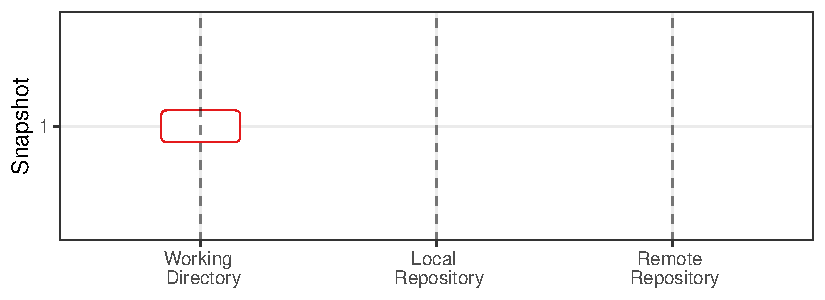
\includegraphics{basics_files/figure-pdf/fig-init-1.pdf}

}

\caption{\label{fig-init}The Git workspace after you have initilized a
repository.}

\end{figure}

\hypertarget{git-add}{%
\subsection{git add}\label{git-add}}

In the last git status report shown above 2 files (\texttt{.gitignore}
and \texttt{git\_practice.Rproj)} were noted that could be added to the
repository. Before we do that let's create third file named fib\_seq.R
which contains a brief header and a single line of code
\texttt{fib\_seq\ \textless{}-\ c(0,\ 1)}. The Fibonacci sequence is the
sequence created when each value in the sequence is the sum of the 2
previous values in the sequence and the vector \texttt{c(0,\ 1)}
initializes the sequence. We will add to this sequence to practice the
use of Git. The terminal session below shows 5 commands: 1) view which
files need to be added with \texttt{git\ status}, 2) add each file one
at a time with \texttt{git\ add}, 3) verify all files have been added
with \texttt{git\ status}. Notice that I made a typo while attempting to
add the \texttt{git\_practice.Rproj} file. I survived this catastrophe
with a warning, which is typical of mistakes in the terminal.

\begin{Shaded}
\begin{Highlighting}[]
\NormalTok{$ git status}
\NormalTok{On branch \{main\}}

\NormalTok{No commits yet}

\NormalTok{Untracked files:}
\NormalTok{  (use "git add \textless{}file\textgreater{}..." to include in what will be committed)}
\NormalTok{        .gitignore}
\NormalTok{        fib\_seq.R}
\NormalTok{        git\_practice.Rproj}

\NormalTok{nothing added to commit but untracked files present (use "git add" to track)}

\NormalTok{amreimer@DFGSXQDSF223076 MINGW64 /s/RTS/Reimer/Research\_Best\_Practices/git\_practice (\{main\})}
\NormalTok{$ git add .gitignore}

\NormalTok{amreimer@DFGSXQDSF223076 MINGW64 /s/RTS/Reimer/Research\_Best\_Practices/git\_practice (\{main\})}
\NormalTok{$ git add fib\_seq.R}

\NormalTok{amreimer@DFGSXQDSF223076 MINGW64 /s/RTS/Reimer/Research\_Best\_Practices/git\_practice (\{main\})}
\NormalTok{$ git\_add git\_practice.Rproj}
\NormalTok{bash: git\_add: command not found}

\NormalTok{amreimer@DFGSXQDSF223076 MINGW64 /s/RTS/Reimer/Research\_Best\_Practices/git\_practice (\{main\})}
\NormalTok{$ git add git\_practice.Rproj}

\NormalTok{amreimer@DFGSXQDSF223076 MINGW64 /s/RTS/Reimer/Research\_Best\_Practices/git\_practice (\{main\})}
\NormalTok{$ git status}
\NormalTok{On branch \{main\}}

\NormalTok{No commits yet}

\NormalTok{Changes to be committed:}
\NormalTok{  (use "git rm {-}{-}cached \textless{}file\textgreater{}..." to unstage)}
\NormalTok{        new file:   .gitignore}
\NormalTok{        new file:   fib\_seq.R}
\NormalTok{        new file:   git\_practice.Rproj}


\NormalTok{amreimer@DFGSXQDSF223076 MINGW64 /s/RTS/Reimer/Research\_Best\_Practices/git\_practice (\{main\})}
\NormalTok{$}
\end{Highlighting}
\end{Shaded}

Use of \texttt{git\ add} stages files you would like to track in your
git repository. The rectangle in Figure~\ref{fig-add} is now filled
which indicates that files within your working directory are staged and
ready to be committed.

\begin{figure}

{\centering 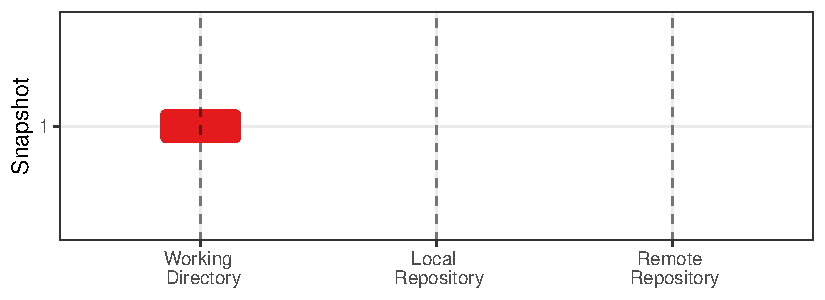
\includegraphics{basics_files/figure-pdf/fig-add-1.pdf}

}

\caption{\label{fig-add}The Git workspace after you have staged files in
your working directory which you intend to add to your local
repository.}

\end{figure}

Notice Git tells you how to unstage a file if you added one
inadvertently. On occasion there are files in your working directory
which you do not want Git to track. Examples might be .pdf files for
literature you referenced while conducting the analysis, word documents
you produced for operational planning and reporting, or extremely large
outputs. It's fine to exclude these sort of files but before you do so
consider\ldots{} ``Would a future researcher need access to this file to
recreate my work?''. If they would you should track them in the
repository.

It can be cumbersome to have a long list of files which Git recognizes
as present in your working directory but you are not actively tracking.
The solution is to open the file .gitignore and include the names of the
files you do not want to track. You can use wildcards if you prefer not
to track all files of a certain type and/or specify folders if you don't
want to track anything in certain sub-directories. For example,
\texttt{*.xlsx} would ignore all .xlsx files in your working directory
while \texttt{posts/} would ignore all of the files in the folder posts
within your working directory.

\hypertarget{git-commit}{%
\subsection{git commit}\label{git-commit}}

In the \texttt{git\ status} response above 3 files were staged. Let's
commit those files in the terminal. In the terminal session below we
verify all of the files we want to commit were staged using
\texttt{git\ status}, recorded (committed) all of the staged files into
the repository using \texttt{git\ commit}, verified the commit worked
using \texttt{git\ status} and examined the repository log using
\texttt{git\ log}.

\begin{Shaded}
\begin{Highlighting}[]
\NormalTok{amreimer@DFGSXQDSF223076 MINGW64 /s/RTS/Reimer/Research\_Best\_Practices/git\_practice (\{main\})}
\NormalTok{$ git status}
\NormalTok{On branch \{main\}}

\NormalTok{No commits yet}

\NormalTok{Changes to be committed:}
\NormalTok{  (use "git rm {-}{-}cached \textless{}file\textgreater{}..." to unstage)}
\NormalTok{        new file:   .gitignore}
\NormalTok{        new file:   fib\_seq.R}
\NormalTok{        new file:   git\_practice.Rproj}


\NormalTok{amreimer@DFGSXQDSF223076 MINGW64 /s/RTS/Reimer/Research\_Best\_Practices/git\_practice (\{main\})}
\NormalTok{$ git commit {-}m "Initialize Fibonacci sequence" {-}m "Sequential additions to the Fibonacci sequence will provide a simple way to demonstrate several cycles of the git workflow including add/commit, push/pull, collaborate, fork, branch, merge, merge conflicts, exc. I even got my wife a GitHub account for this. Wish us luck!"}
\NormalTok{[\{main\} e17181f] Initialize Fibonacci sequence}
\NormalTok{ Date: Sun Jul 2 12:59:06 2023 {-}0800}
\NormalTok{ 3 files changed, 21 insertions(+)}
\NormalTok{ create mode 100644 .gitignore}
\NormalTok{ create mode 100644 fib\_seq.R}
\NormalTok{ create mode 100644 git\_practice.Rproj}

\NormalTok{amreimer@DFGSXQDSF223076 MINGW64 /s/RTS/Reimer/Research\_Best\_Practices/git\_practice (\{main\})}
\NormalTok{$ git status}
\NormalTok{On branch \{main\}}
\NormalTok{nothing to commit, working tree clean}

\NormalTok{amreimer@DFGSXQDSF223076 MINGW64 /s/RTS/Reimer/Research\_Best\_Practices/git\_practice (\{main\})}
\NormalTok{$ git log}
\NormalTok{commit e17181fa781b2e30096e1c7d31443aac18d527e5 (HEAD {-}\textgreater{} \{main\})}
\NormalTok{Author: Adam Reimer \textless{}adam.reimer@alaska.gov\textgreater{}}
\NormalTok{Date:   Sun Jul 2 12:59:06 2023 {-}0800}

\NormalTok{    Initialize Fibonacci sequence}

\NormalTok{    Sequential additions to the Fibonacci sequence will provide a simple way to demonstrate several cycles of the git workflow including add/commit, push/pull, collaborate, fork, branch, merge, merge conflicts, exc. I even got my wife a GitHub account for this. Wish us luck!}

\NormalTok{amreimer@DFGSXQDSF223076 MINGW64 /s/RTS/Reimer/Research\_Best\_Practices/git\_practice (\{main\})}
\NormalTok{$}
\end{Highlighting}
\end{Shaded}

The \texttt{git\ log} command provides a summary of the commit. Two
important parts are the commit ID and the commit message. The commit ID
is a code which can be used to reference the commit in the future. Git
assigned a long ID to each commit
(\texttt{e17181fa781b2e30096e1c7d31443aac18d527e5} for this commit) but
its common to using only the first 7 characters of the commit ID
(\texttt{e17181f)} to refer to the commit.

Commit messages are required. Notice the commit message is broken into 2
parts. The first part is called the title or summary while the second
part is called the description. A good practice is for the title to be
brief (less that 50 characters) so that it displays well in most
formats. There is no length limit for the description and this is the
place to provide some explanation beyond what you can capture in the
title. I've purposely been verbose with the commit above to demonstrate
a long description.

\begin{figure}

{\centering 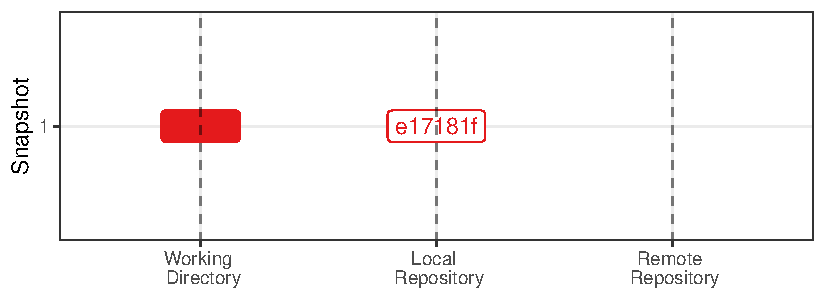
\includegraphics{basics_files/figure-pdf/fig-push-1.pdf}

}

\caption{\label{fig-push}The Git workspace after you have committed your
staged files to your local repository.}

\end{figure}

The git workflow described so far forms the basis on reproducible
research using Git. We will calculate the next several values in the
Fibonacci sequence to practice this workflow. The same sqence described
above is repeated:

\begin{enumerate}
\def\labelenumi{\arabic{enumi}.}
\item
  A change is made to \texttt{fib\_seq.R} (in this case a new line
  \texttt{fib\_seq{[}3{]}\ \textless{}-\ fib\_seq{[}1{]}\ +\ fib\_seq{[}2{]}}
  is added) and saved to the working directory. Te working directory now
  represents a more recent snapshot of time that the local repository.
\item
  The changed file is staged.
\item
  The staged file is committed.
\item
  Repeat steps 1 through 3.
\end{enumerate}

The process looks like:

\begin{figure}

\begin{minipage}[t]{0.50\linewidth}

{\centering 

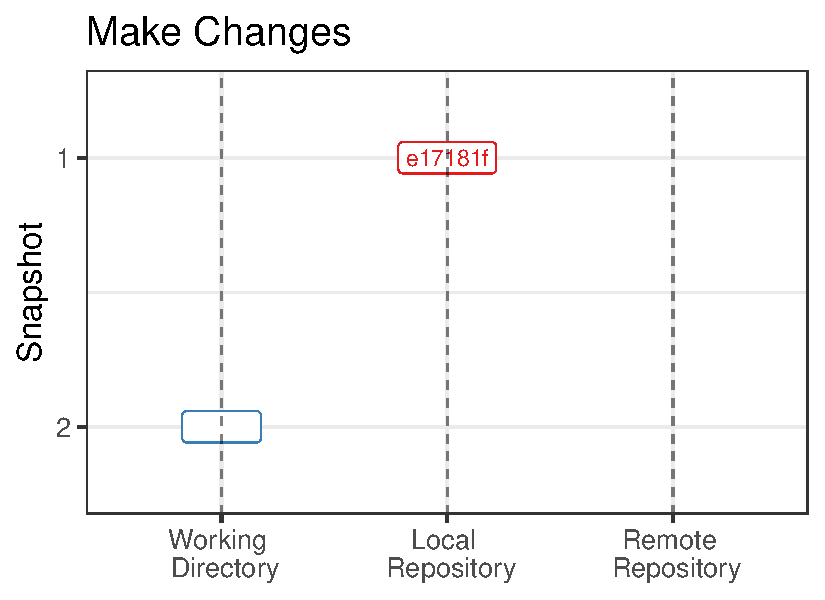
\includegraphics{basics_files/figure-pdf/unnamed-chunk-7-1.pdf}

}

\end{minipage}%
%
\begin{minipage}[t]{0.50\linewidth}

{\centering 

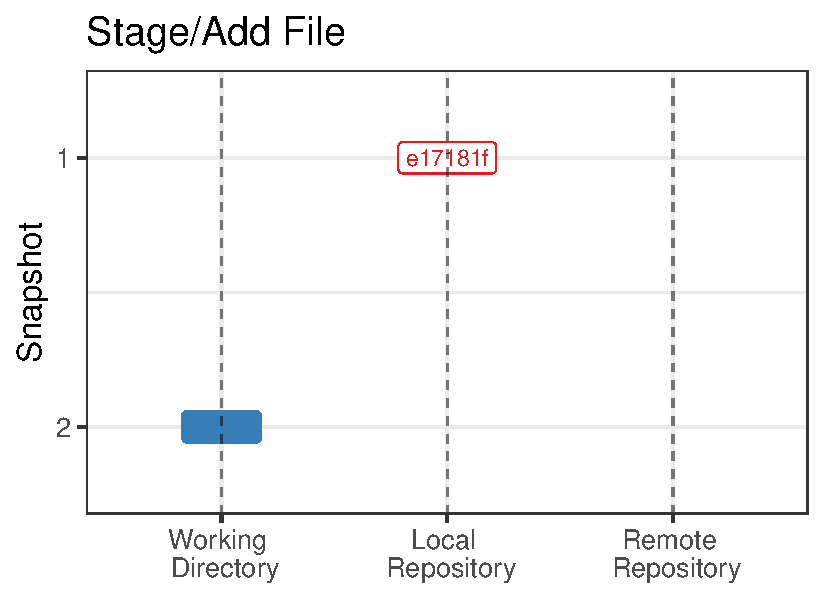
\includegraphics{basics_files/figure-pdf/unnamed-chunk-8-1.pdf}

}

\end{minipage}%
\newline
\begin{minipage}[t]{0.50\linewidth}

{\centering 

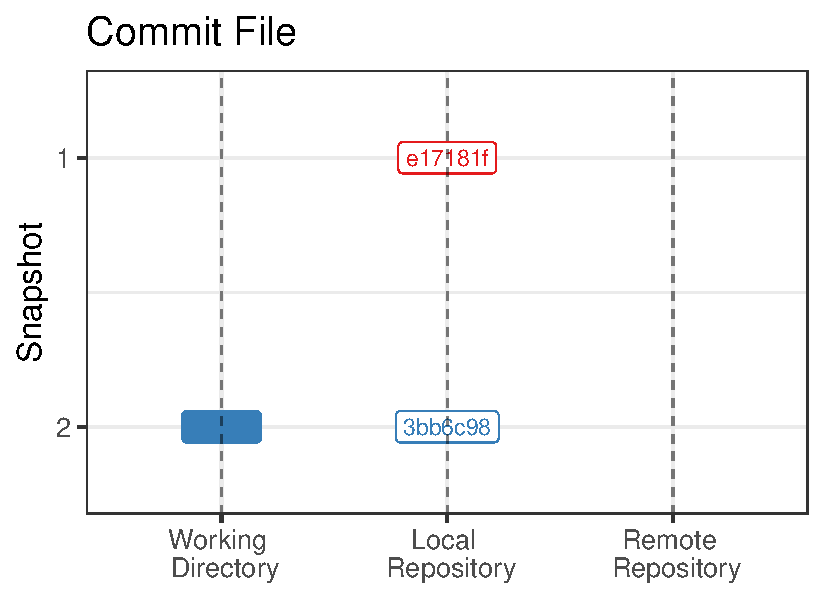
\includegraphics{basics_files/figure-pdf/unnamed-chunk-9-1.pdf}

}

\end{minipage}%
%
\begin{minipage}[t]{0.50\linewidth}

{\centering 

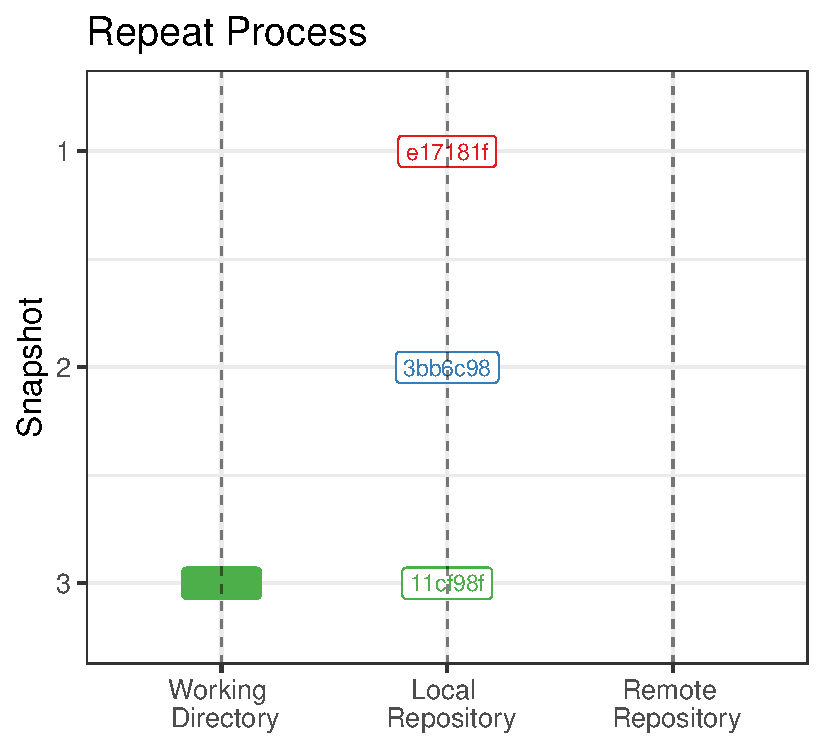
\includegraphics{basics_files/figure-pdf/unnamed-chunk-10-1.pdf}

}

\end{minipage}%

\end{figure}

\hypertarget{when-to-commit}{%
\subsubsection{When to Commit?}\label{when-to-commit}}

Saves and a commits serve different purposes. As we all know, save can
and should be used frequently\ldots{} many times an hour and/or any time
you are stepping away from your work. This use is agnostic to whether
the analyst is or is not using a git workflow.

In contrast, commits are made for two reasons. First, a commit should be
made whenever the analysis is at a point which you may want to revisit.
Examples include; adding new data, adding a new feature to the analysis,
or any time the code was run and the results were distributed. Any one
of these tasks may have resulted in a new `version' in the traditional
workflow but they don't have to be major updates. A second reason to
commit is when the changes are substantive enough that the line-by-line
change may be difficult to track if you did not commit until the new
data/feature are complete. These commits snapshot significant steps in a
new feature's development or prior to experimenting with a new feature.

The most important thing to note regarding commits is that, unlike save,
there is no temporal component. While saves are designed to minimize the
risk of lost work and should be frequent \emph{in time}, commits are
designed to record importance stages of the analysis and should be
frequent \emph{with respect to progress}. A difficult feature may take
days to code but represent a single commit, provided the actual changes
to the code are modest. Efficiency in commit frequency will pay off when
the repository is being revisited at a later date and each commit is a
snapshot of the analysis that is important or informative to the
reviewer.

\hypertarget{git-log}{%
\subsection{git log}\label{git-log}}

To view our commit history in the terminal use \texttt{git\ log}. Note
that the commit ID, author, date, commit title and commit description
are all shown in the log.

\begin{Shaded}
\begin{Highlighting}[]
\NormalTok{amreimer@DFGSXQDSF223076 MINGW64 /s/RTS/Reimer/Research\_Best\_Practices/git\_practice (\{main\})}
\NormalTok{$ git log}
\NormalTok{commit 11cf98ff67b8ec4f8cd7f2c1650a176d5875fdcf (HEAD {-}\textgreater{} \{main\})}
\NormalTok{Author: Adam Reimer \textless{}adam.reimer@alaska.gov\textgreater{}}
\NormalTok{Date:   Sun Jul 2 14:53:05 2023 {-}0800}

\NormalTok{    Fourth entry in the Fibonacci sequence}

\NormalTok{    Long and informative message goes here.}

\NormalTok{commit 3bb6c98bb0048bad7bda489bd8d40be24fb66acf}
\NormalTok{Author: Adam Reimer \textless{}adam.reimer@alaska.gov\textgreater{}}
\NormalTok{Date:   Sun Jul 2 14:31:04 2023 {-}0800}

\NormalTok{    Third entry in fib\_seq}

\NormalTok{    This message is not necessary for such a simple commit, but descriptions are an important part of reproducible research I’m writing a long message to set a good example.  Have better content in yours.}

\NormalTok{commit e17181fa781b2e30096e1c7d31443aac18d527e5}
\NormalTok{Author: Adam Reimer \textless{}adam.reimer@alaska.gov\textgreater{}}
\NormalTok{Date:   Sun Jul 2 12:59:06 2023 {-}0800}

\NormalTok{    Initialize Fibonacci sequence}

\NormalTok{    Sequential additions to the Fibonacci sequence will provide a simple way to demonstrate several cycles of the git workflow including add/commit, push/pull, collaborate, fork, branch, merge, merge conflicts, exc. I even got my wife a GitHub account}
\NormalTok{for this. Wish us luck!}

\NormalTok{amreimer@DFGSXQDSF223076 MINGW64 /s/RTS/Reimer/Research\_Best\_Practices/git\_practice (\{main\})}
\NormalTok{$}
\end{Highlighting}
\end{Shaded}

\hypertarget{git-diff}{%
\subsection{git diff}\label{git-diff}}

To see the difference between two commits use \texttt{git\ diff}. With
no additional arguments \texttt{git\ diff} will show the changes in the
working directory relative to the last commit. Our working directory has
no changes as illustrated by \texttt{git\ status}. Instead we can add a
short commit ID to the command to see changed between the current
working directory and the commit \texttt{3bb6c9}.

\begin{Shaded}
\begin{Highlighting}[]
\NormalTok{amreimer@DFGSXQDSF223076 MINGW64 /s/RTS/Reimer/Research\_Best\_Practices/git\_practice (\{main\})}
\NormalTok{$ git status}
\NormalTok{On branch \{main\}}
\NormalTok{nothing to commit, working tree clean}

\NormalTok{amreimer@DFGSXQDSF223076 MINGW64 /s/RTS/Reimer/Research\_Best\_Practices/git\_practice (\{main\})}
\NormalTok{$ git diff 3bb6c9}
\NormalTok{diff {-}{-}git a/fib\_seq.R b/fib\_seq.R}
\NormalTok{index 9c118d5..4ce1d70 100644}
\NormalTok{{-}{-}{-} a/fib\_seq.R}
\NormalTok{+++ b/fib\_seq.R}
\NormalTok{@@ {-}2,4 +2,5 @@}
\NormalTok{ \#Adam Reimer}

\NormalTok{ fib\_seq \textless{}{-} c(0, 1)}
\NormalTok{{-}fib\_seq[3] \textless{}{-} fib\_seq[1] + fib\_seq[2]}
\NormalTok{\textbackslash{} No newline at end of file}
\NormalTok{+fib\_seq[3] \textless{}{-} fib\_seq[1] + fib\_seq[2]}
\NormalTok{+fib\_seq[4] \textless{}{-} fib\_seq[2] + fib\_seq[3]}
\NormalTok{\textbackslash{} No newline at end of file}

\NormalTok{amreimer@DFGSXQDSF223076 MINGW64 /s/RTS/Reimer/Research\_Best\_Practices/git\_practice (\{main\})}
\NormalTok{$}
\end{Highlighting}
\end{Shaded}

Git GUI's are superior to the terminal when looking at line-by line
differences but for completeness we will discuss how to read the output.
The section \texttt{-\/-\/-\ a/fib\_seq.R} to \texttt{+++\ b/fib\_seq.R}
identifies the files that were modified where \texttt{-\/-\/-\ a/} and
\texttt{+++\ b} refer to the previous and the current versions of the
file respectively. The line \texttt{@@\ -2,4\ +2,5\ @@} tells us that
the output is showing the original file starting on the second line and
displaying the the next 4 lines (three unmarked lines and the line with
a negative symbol) while the new version of the file is also shown
starting from the second line but displaying the next 5 lines (the three
unmarked lines and the two lines with an addition symbol). This makes
sense because a single line was added to the new version.

\bookmarksetup{startatroot}

\hypertarget{collaboration-using-git}{%
\chapter{Collaboration Using Git}\label{collaboration-using-git}}

Git has some amazing reproducible research capabilities that can become
really powerful in large complicated analyses. That said, utilizing Git
comes with an overhead that may not be justified for small projects
unless you consider collaboration with future analysts including
yourself. To demonstrate Git's collaborative potential I created a
remote repository on GitHub called git\_practice.

\hypertarget{interacting-with-your-remote-repository}{%
\subsection{Interacting with your Remote
Repository}\label{interacting-with-your-remote-repository}}

\hypertarget{git-push}{%
\subsubsection{git push}\label{git-push}}

To link your local repository to a remote repository use
\texttt{git\ remote}. In the terminal session below I added a remote
repository named ``origin'' and provided a url where the repository is
located. The second command created a new branch in the remote named
\texttt{main}. The third command ``pushed'' my local repository to my
remote repository. Files associated with this repository are now stored
in a location where they can be accessed by others for viewing,
download, or collaborative work.

\begin{Shaded}
\begin{Highlighting}[]
\NormalTok{amreimer@DFGSXQDSF223076 MINGW64 /s/RTS/Reimer/Research\_Best\_Practices/git\_practice (\{main\})}
\NormalTok{$ git remote add origin https://github.com/adamreimer/git\_practice.git}

\NormalTok{amreimer@DFGSXQDSF223076 MINGW64 /s/RTS/Reimer/Research\_Best\_Practices/git\_practice (\{main\})}
\NormalTok{$ git branch {-}M main}

\NormalTok{amreimer@DFGSXQDSF223076 MINGW64 /s/RTS/Reimer/Research\_Best\_Practices/git\_practice (main)}
\NormalTok{$ git push {-}u origin main}
\NormalTok{Enumerating objects: 11, done.}
\NormalTok{Counting objects: 100\% (11/11), done.}
\NormalTok{Delta compression using up to 16 threads}
\NormalTok{Compressing objects: 100\% (10/10), done.}
\NormalTok{Writing objects: 100\% (11/11), 1.53 KiB | 8.00 KiB/s, done.}
\NormalTok{Total 11 (delta 2), reused 0 (delta 0), pack{-}reused 0}
\NormalTok{remote: Resolving deltas: 100\% (2/2), done.}
\NormalTok{To https://github.com/adamreimer/git\_practice.git}
\NormalTok{ * [new branch]      main {-}\textgreater{} main}
\NormalTok{branch \textquotesingle{}main\textquotesingle{} set up to track \textquotesingle{}origin/main\textquotesingle{}.}

\NormalTok{amreimer@DFGSXQDSF223076 MINGW64 /s/RTS/Reimer/Research\_Best\_Practices/git\_practice (main)}
\NormalTok{$}
\end{Highlighting}
\end{Shaded}

After pushing to github your repository now looks like
Figure~\ref{fig-push}.

\begin{figure}

{\centering 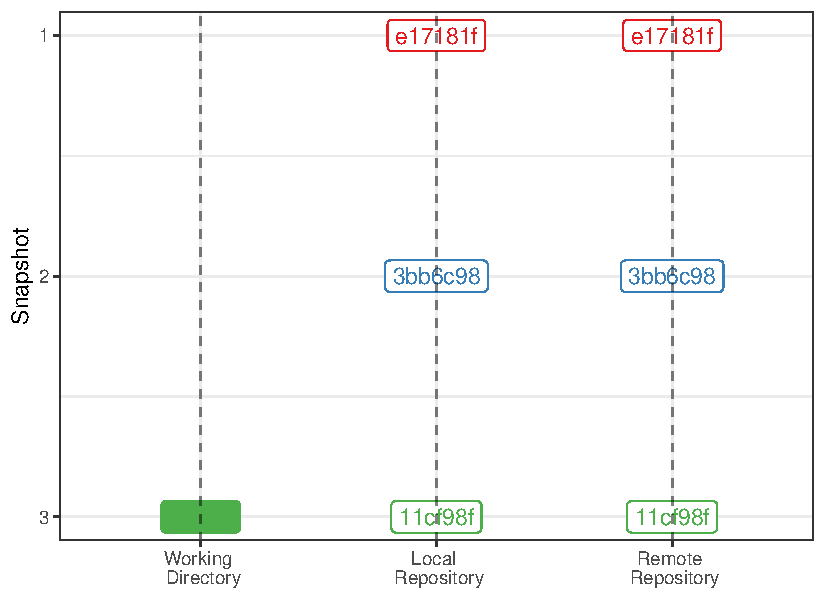
\includegraphics{collaboration_files/figure-pdf/fig-push-1.pdf}

}

\caption{\label{fig-push}The Git workspace after your local repository
has been pushed to a remote repository.}

\end{figure}

Now that we have a remote repository updated we have to worry about
keeping them both synced. To illustrate this workflow I'll change the
\texttt{fib\_seq.r} file by adding the fifth value to the Fibonacci
sequence
(\texttt{fib\_seq{[}5{]}\ \textless{}-\ fib\_seq{[}3{]}\ +\ fib\_seq{[}4{]}})
as a new line. After this change the git work space will contain an
unstaged change which is not reflected in either repository.

\begin{figure}

{\centering 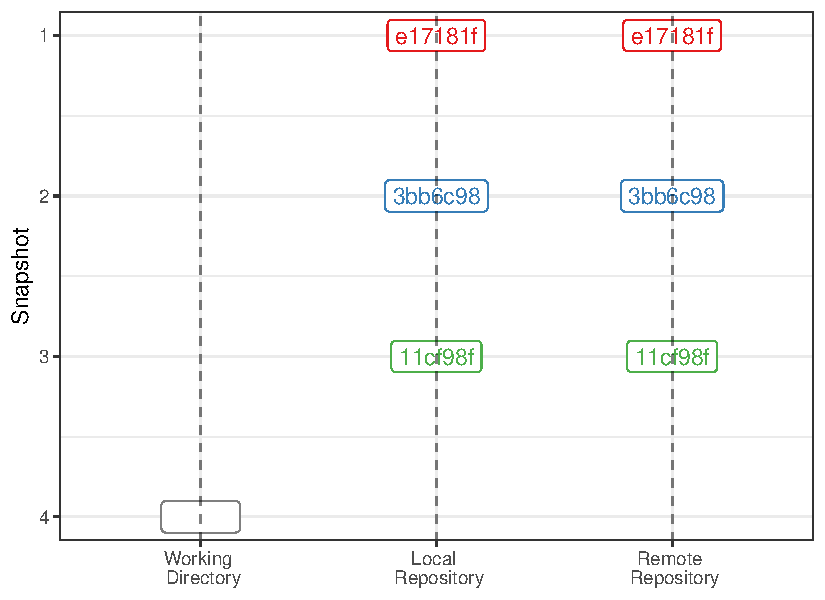
\includegraphics{collaboration_files/figure-pdf/fig-changewremote-1.pdf}

}

\caption{\label{fig-changewremote}The Git workspace after the working
directory has been changed leaving the local and remote repositories
out-of-date.}

\end{figure}

In the terminal session below I stage the file \texttt{fib\_seq.R} and
commit the file. Notice the first time we submitted a
\texttt{git\ status} command we were told the local and remote
repositories were synced but that there were unstaged changes. After the
modified file was added and committed the second call to
\texttt{git\ status} tells us our remote repository is one commit behind
our local repository. The git work space at this moment is illustrated
by Figure~\ref{fig-commitwremote}.

\begin{Shaded}
\begin{Highlighting}[]
\NormalTok{amreimer@DFGSXQDSF223076 MINGW64 /s/RTS/Reimer/Research\_Best\_Practices/git\_practice (main)}
\NormalTok{$ git status}
\NormalTok{On branch main}
\NormalTok{Your branch is up to date with \textquotesingle{}origin/main\textquotesingle{}.}

\NormalTok{Changes not staged for commit:}
\NormalTok{  (use "git add \textless{}file\textgreater{}..." to update what will be committed)}
\NormalTok{  (use "git restore \textless{}file\textgreater{}..." to discard changes in working directory)}
\NormalTok{        modified:   fib\_seq.R}

\NormalTok{no changes added to commit (use "git add" and/or "git commit {-}a")}

\NormalTok{amreimer@DFGSXQDSF223076 MINGW64 /s/RTS/Reimer/Research\_Best\_Practices/git\_practice (main)}
\NormalTok{$ git add fib\_seq.R}

\NormalTok{amreimer@DFGSXQDSF223076 MINGW64 /s/RTS/Reimer/Research\_Best\_Practices/git\_practice (main)}
\NormalTok{$ git commit {-}m "Fifth entry in the Fibonacci sequence" {-}m "A long and descriptive description"}
\NormalTok{[main 5139049] Fifth entry in the Fibonacci sequence}
\NormalTok{ 1 file changed, 2 insertions(+), 1 deletion({-})}

\NormalTok{amreimer@DFGSXQDSF223076 MINGW64 /s/RTS/Reimer/Research\_Best\_Practices/git\_practice (main)}
\NormalTok{$ git status}
\NormalTok{On branch main}
\NormalTok{Your branch is ahead of \textquotesingle{}origin/main\textquotesingle{} by 1 commit.}
\NormalTok{  (use "git push" to publish your local commits)}

\NormalTok{nothing to commit, working tree clean}

\NormalTok{amreimer@DFGSXQDSF223076 MINGW64 /s/RTS/Reimer/Research\_Best\_Practices/git\_practice (main)}
\NormalTok{$}
\end{Highlighting}
\end{Shaded}

\begin{figure}

{\centering 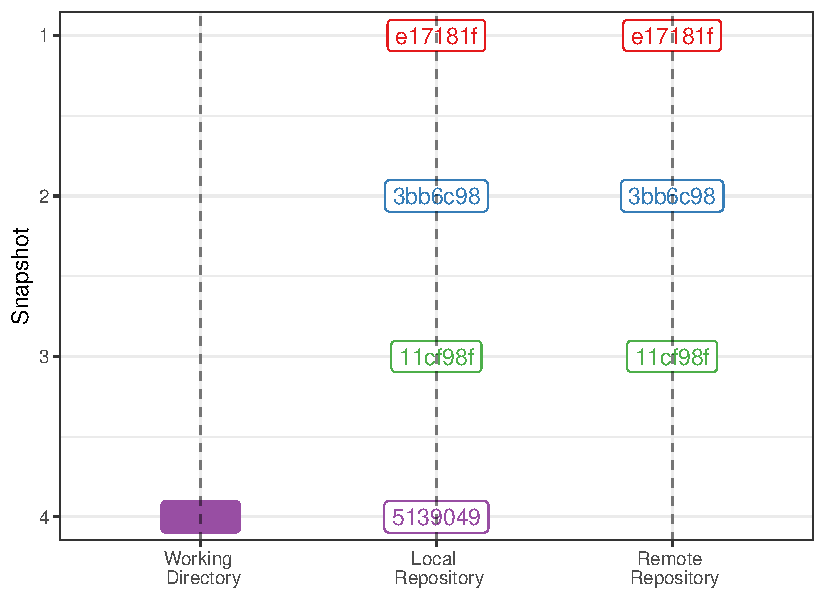
\includegraphics{collaboration_files/figure-pdf/fig-commitwremote-1.pdf}

}

\caption{\label{fig-commitwremote}The Git workspace after a local change
has been staged \& committed leaving the remote repositories one commit
behind.}

\end{figure}

In the terminal session below I use \texttt{git\ push} to update the
remote repository. Notice \texttt{git\ status} verifies the repositories
are now synced. The git work space at this moment is illustrated by
Figure~\ref{fig-pushwremote}.

\begin{Shaded}
\begin{Highlighting}[]
\NormalTok{amreimer@DFGSXQDSF223076 MINGW64 /s/RTS/Reimer/Research\_Best\_Practices/git\_practice (main)}
\NormalTok{$ git push}
\NormalTok{Enumerating objects: 5, done.}
\NormalTok{Counting objects: 100\% (5/5), done.}
\NormalTok{Delta compression using up to 16 threads}
\NormalTok{Compressing objects: 100\% (3/3), done.}
\NormalTok{Writing objects: 100\% (3/3), 414 bytes | 8.00 KiB/s, done.}
\NormalTok{Total 3 (delta 1), reused 0 (delta 0), pack{-}reused 0}
\NormalTok{remote: Resolving deltas: 100\% (1/1), completed with 1 local object.}
\NormalTok{To https://github.com/adamreimer/git\_practice.git}
\NormalTok{   0c92881..5139049  main {-}\textgreater{} main}

\NormalTok{amreimer@DFGSXQDSF223076 MINGW64 /s/RTS/Reimer/Research\_Best\_Practices/git\_practice (main)}
\NormalTok{$ git status}
\NormalTok{On branch main}
\NormalTok{Your branch is up to date with \textquotesingle{}origin/main\textquotesingle{}.}

\NormalTok{nothing to commit, working tree clean}

\NormalTok{amreimer@DFGSXQDSF223076 MINGW64 /s/RTS/Reimer/Research\_Best\_Practices/git\_practice (main)}
\NormalTok{$}
\end{Highlighting}
\end{Shaded}

\begin{figure}

{\centering 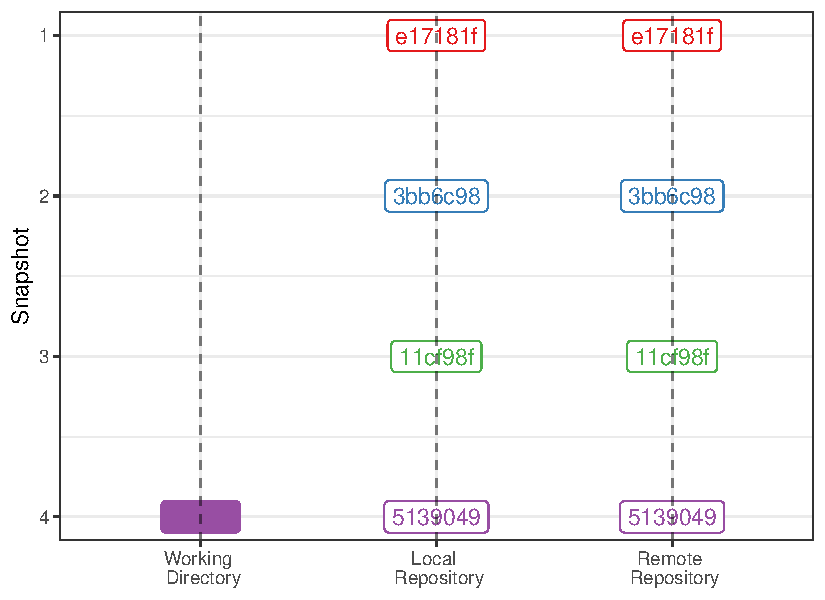
\includegraphics{collaboration_files/figure-pdf/fig-pushwremote-1.pdf}

}

\caption{\label{fig-pushwremote}The Git workspace after a local change
has been staged, committed, and pushed.}

\end{figure}

\hypertarget{git-clone}{%
\subsubsection{git clone}\label{git-clone}}

Imagine a situation where you would like to work on your analysis from a
home computer\footnote{I hope your analysis is on the network and you
  could use vpn to solve this problem.}. If your analysis is stored as a
git repository it is easy to obtain a copy from a different computer. In
the terminal sequence below we navigate to my home computer's C drive,
clone the remote repository to the C drive, navigate to the new local
repository, and check the repository status. Notice that I made a typo
on the \texttt{git\ status} command the first time and nothing terrible
happened.

\begin{Shaded}
\begin{Highlighting}[]
\NormalTok{amreimer@DFGSXQDSF223076 MINGW64 \textasciitilde{}/Documents}
\NormalTok{$ cd C:/}

\NormalTok{amreimer@DFGSXQDSF223076 MINGW64 /c}
\NormalTok{$ git clone https://github.com/adamreimer/git\_practice.git}
\NormalTok{Cloning into \textquotesingle{}git\_practice\textquotesingle{}...}
\NormalTok{remote: Enumerating objects: 14, done.}
\NormalTok{remote: Counting objects: 100\% (14/14), done.}
\NormalTok{remote: Compressing objects: 100\% (10/10), done.}
\NormalTok{remote: Total 14 (delta 3), reused 14 (delta 3), pack{-}reused 0}
\NormalTok{Receiving objects: 100\% (14/14), done.}
\NormalTok{Resolving deltas: 100\% (3/3), done.}

\NormalTok{amreimer@DFGSXQDSF223076 MINGW64 /c}
\NormalTok{$ cd C:/git\_practice}

\NormalTok{amreimer@DFGSXQDSF223076 MINGW64 /c/git\_practice (main)}
\NormalTok{$ git\_status}
\NormalTok{bash: git\_status: command not found}

\NormalTok{amreimer@DFGSXQDSF223076 MINGW64 /c/git\_practice (main)}
\NormalTok{$ git status}
\NormalTok{On branch main}
\NormalTok{Your branch is up to date with \textquotesingle{}origin/main\textquotesingle{}.}

\NormalTok{nothing to commit, working tree clean}

\NormalTok{amreimer@DFGSXQDSF223076 MINGW64 /c/git\_practice (main)}
\NormalTok{$}
\end{Highlighting}
\end{Shaded}

After \texttt{git\ clone} the my remote repository to my home machine I
have two local repositories associated with the same remote(see
Figure~\ref{fig-home}).

\begin{figure}

{\centering 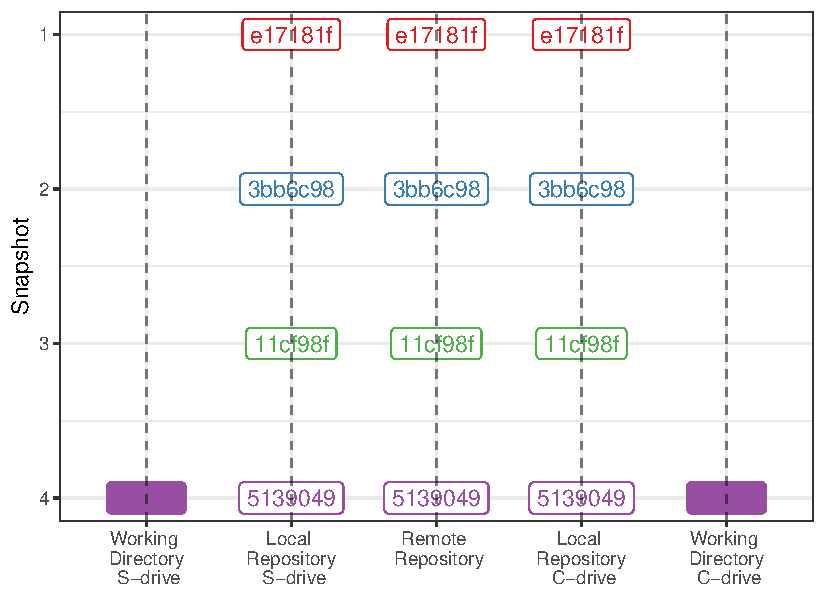
\includegraphics{collaboration_files/figure-pdf/fig-home-1.pdf}

}

\caption{\label{fig-home}The Git workspace when you have two local
repositories associated with the same remote.}

\end{figure}

If I change the file \texttt{fib\_seq.R} in the working directory of my
home computer by adding a new line
(\texttt{fib\_seq{[}6{]}\ \textless{}-\ fib\_seq{[}4{]}\ +\ fib\_seq{[}5{]}}),
stage and commit those changes in the local repository on my home
computer, and push my home computer's local repository to the remote
repository the local repository on my S drive to be behind one commit.
The terminal session below demonstrated these commands (all of which we
have seen before) and the current state of the Git work space is shown
in Figure~\ref{fig-homeahead}.

\begin{Shaded}
\begin{Highlighting}[]
\NormalTok{amreimer@DFGSXQDSF223076 MINGW64 /c/git\_practice (main)}
\NormalTok{$ git status}
\NormalTok{On branch main}
\NormalTok{Your branch is up to date with \textquotesingle{}origin/main\textquotesingle{}.}

\NormalTok{Changes not staged for commit:}
\NormalTok{  (use "git add \textless{}file\textgreater{}..." to update what will be committed)}
\NormalTok{  (use "git restore \textless{}file\textgreater{}..." to discard changes in working directory)}
\NormalTok{        modified:   fib\_seq.R}

\NormalTok{no changes added to commit (use "git add" and/or "git commit {-}a")}

\NormalTok{amreimer@DFGSXQDSF223076 MINGW64 /c/git\_practice (main)}
\NormalTok{$ git add fib\_seq.R}

\NormalTok{amreimer@DFGSXQDSF223076 MINGW64 /c/git\_practice (main)}
\NormalTok{$ git commit {-}m "Sixth number in the Fibonacci seqence" {-}m "This commit is slightly different as it was made from a different computer in my house. It still represents a single author working on their own repository but demonstrated the flexibility accorded by storing your analysis on the cloud. Working on this analysis from a new machine was seamless provided the new machine had the appropriate software."}
\NormalTok{[main 9db5478] Sixth number in the Fibonacci seqence}
\NormalTok{ 1 file changed, 2 insertions(+), 1 deletion({-})}

\NormalTok{amreimer@DFGSXQDSF223076 MINGW64 /c/git\_practice (main)}
\NormalTok{$ git status}
\NormalTok{On branch main}
\NormalTok{Your branch is ahead of \textquotesingle{}origin/main\textquotesingle{} by 1 commit.}
\NormalTok{  (use "git push" to publish your local commits)}

\NormalTok{nothing to commit, working tree clean}

\NormalTok{amreimer@DFGSXQDSF223076 MINGW64 /c/git\_practice (main)}
\NormalTok{$ git push}
\NormalTok{Enumerating objects: 5, done.}
\NormalTok{Counting objects: 100\% (5/5), done.}
\NormalTok{Delta compression using up to 16 threads}
\NormalTok{Compressing objects: 100\% (3/3), done.}
\NormalTok{Writing objects: 100\% (3/3), 586 bytes | 586.00 KiB/s, done.}
\NormalTok{Total 3 (delta 1), reused 0 (delta 0), pack{-}reused 0}
\NormalTok{remote: Resolving deltas: 100\% (1/1), completed with 1 local object.}
\NormalTok{To https://github.com/adamreimer/git\_practice.git}
\NormalTok{   5139049..9db5478  main {-}\textgreater{} main}

\NormalTok{amreimer@DFGSXQDSF223076 MINGW64 /c/git\_practice (main)}
\NormalTok{$}
\end{Highlighting}
\end{Shaded}

\begin{figure}

{\centering 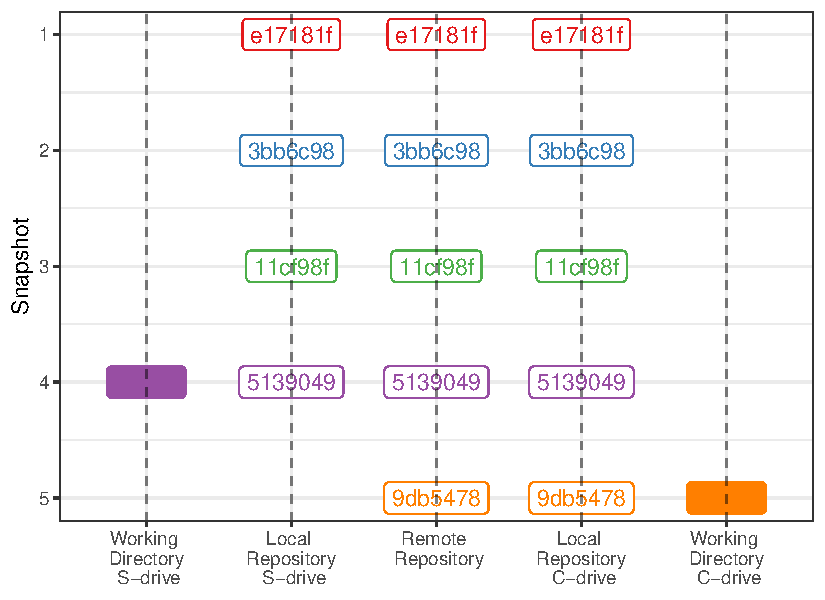
\includegraphics{collaboration_files/figure-pdf/fig-homeahead-1.pdf}

}

\caption{\label{fig-homeahead}The Git workspace when you have one local
repository has pushed a new commit to the remote repository.}

\end{figure}

\hypertarget{git-pull}{%
\subsubsection{git pull}\label{git-pull}}

As Figure~\ref{fig-homeahead} demonstrate the local repository on my S
drive is now one commit behind the remote (and the local repository on
my C drive). In the terminal session below we try \texttt{git\ status}
but are told the local and remote repositories are synced, which we know
to be false. Git has lost track of the remote since the repository on
the S drive was blind to the last commit. Instead we use
\texttt{git\ update} to update the remote connection, after which git
status works as before. Finally, \texttt{git\ pull} brings the local
repository on the S drive into sync with the remote. At this point the
local and remote repositories have the structure of
Figure~\ref{fig-home} but will include an additional commit
(\texttt{9db5478}) not shown in Figure~\ref{fig-home}.

\begin{Shaded}
\begin{Highlighting}[]
\NormalTok{amreimer@DFGSXQDSF223076 MINGW64 /s/RTS/Reimer/Research\_Best\_Practices/git\_practice (main)}
\NormalTok{$ git status}
\NormalTok{On branch main}
\NormalTok{Your branch is up to date with \textquotesingle{}origin/main\textquotesingle{}.}

\NormalTok{nothing to commit, working tree clean}

\NormalTok{amreimer@DFGSXQDSF223076 MINGW64 /s/RTS/Reimer/Research\_Best\_Practices/git\_practice (main)}
\NormalTok{$ git remote update}
\NormalTok{remote: Enumerating objects: 5, done.}
\NormalTok{remote: Counting objects: 100\% (5/5), done.}
\NormalTok{remote: Compressing objects: 100\% (2/2), done.}
\NormalTok{remote: Total 3 (delta 1), reused 3 (delta 1), pack{-}reused 0}
\NormalTok{Unpacking objects: 100\% (3/3), 566 bytes | 0 bytes/s, done.}
\NormalTok{From https://github.com/adamreimer/git\_practice}
\NormalTok{   5139049..9db5478  main       {-}\textgreater{} origin/main}

\NormalTok{amreimer@DFGSXQDSF223076 MINGW64 /s/RTS/Reimer/Research\_Best\_Practices/git\_practice (main)}
\NormalTok{$ git status}
\NormalTok{On branch main}
\NormalTok{Your branch is behind \textquotesingle{}origin/main\textquotesingle{} by 1 commit, and can be fast{-}forwarded.}
\NormalTok{  (use "git pull" to update your local branch)}

\NormalTok{nothing to commit, working tree clean}

\NormalTok{amreimer@DFGSXQDSF223076 MINGW64 /s/RTS/Reimer/Research\_Best\_Practices/git\_practice (main)}
\NormalTok{$ git pull}
\NormalTok{Updating 5139049..9db5478}
\NormalTok{Fast{-}forward}
\NormalTok{ fib\_seq.R | 3 ++{-}}
\NormalTok{ 1 file changed, 2 insertions(+), 1 deletion({-})}

\NormalTok{amreimer@DFGSXQDSF223076 MINGW64 /s/RTS/Reimer/Research\_Best\_Practices/git\_practice (main)}
\NormalTok{$ git status}
\NormalTok{On branch main}
\NormalTok{Your branch is up to date with \textquotesingle{}origin/main\textquotesingle{}.}

\NormalTok{nothing to commit, working tree clean}

\NormalTok{amreimer@DFGSXQDSF223076 MINGW64 /s/RTS/Reimer/Research\_Best\_Practices/git\_practice (main)}
\NormalTok{$}
\end{Highlighting}
\end{Shaded}

\hypertarget{interacting-with-a-peers-remote-repository}{%
\subsection{Interacting with a Peer's Remote
Repository}\label{interacting-with-a-peers-remote-repository}}

How you interact with a peers remote repository depends on your goals.
We will discuss three typical use cases below.

\hypertarget{git-clone---to-copymodify-code}{%
\subsubsection{git clone - To Copy/Modify
Code}\label{git-clone---to-copymodify-code}}

Imagine a situation where a peer has written some code which you would
like to modify for a similar project\footnote{Common courtesy requires
  you to ask permission and credit the person who originally wrote the
  code.}. Use \texttt{git\ clone} as described above. You will be able
to create a copy of their repository and work on your local machine as
usual, but you will not be able to push changes back to the remote.

\hypertarget{git-clone-git-push-git-pull---to-collaborate-closely}{%
\subsubsection{git clone, git push, git pull - To Collaborate
(closely)}\label{git-clone-git-push-git-pull---to-collaborate-closely}}

If you and a peer are working closely on a analysis it may be
appropriate for the owner to add their peer as a collaborator to the
project. This is a point-and-click task from your github repository
page, \emph{Settings\textgreater Collaborators\textgreater Add
people\textgreater(keypunch the username}). The collaborator can push
and pull changes to the remote as if they were the owner. This
arraignment is only appropriate for peers who you trust to commit
changes of which you both approve. In practice, this likely means there
will be personal communication to coordinate each person's efforts. To
demonstrate this process I added my wife (Carly) as a collaborator to
the git\_practice repository. Carly then cloned the repository, modified
the \texttt{fib\_seq.R} file by adding a new line
(\texttt{fib\_seq{[}7{]}\ \textless{}-\ fib\_seq{[}5{]}\ +\ fib\_seq{[}6{]}}),
staged the file, committed the changes, and pushed her local repository
back to the git\_practice remote. Afterwards I pulled those changes back
to the local repository on my S drive. The terminal sessions and figures
associated with these actions would closely mirror those shown for
\texttt{git\ clone}, \texttt{git\ push}, and \texttt{git\ pull} above
although the local repositories have different owners in this case. To
demonstrate commits were made by both collaborators I ran a specially
formatted call\footnote{Thanks
  \href{https://stackoverflow.com/questions/1441010/the-shortest-possible-output-from-git-log-containing-author-and-date}{Jesper
  Rønn-Jensen}! Note: \%h specifies the short commit ID, \%x09 specifies
  a tab, \%an specifies the author, \%ad specifies the commit date, and
  \%s specifies the commit title.} to \texttt{git\ log} which shows that
the latest commit to this repository did come form a new author.

\begin{Shaded}
\begin{Highlighting}[]
\NormalTok{amreimer@DFGSXQDSF223076 MINGW64 /s/RTS/Reimer/Research\_Best\_Practices/git\_practice (main)}
\NormalTok{$ git log {-}{-}pretty=format:"\%h\%x09\%an\%x09\%ad\%x09\%s"}
\NormalTok{f732cdb Carly Reimer    Sun Jul 2 22:01:17 2023 {-}0800   Seventh Fibonacci number}
\NormalTok{9db5478 Adam Reimer     Sun Jul 2 20:39:19 2023 {-}0800   Sixth number in the Fibonacci seqence}
\NormalTok{5139049 Adam Reimer     Sun Jul 2 16:15:52 2023 {-}0800   Fifth entry in the Fibonacci sequence}
\NormalTok{0c92881 Adam Reimer     Sun Jul 2 14:53:05 2023 {-}0800   Fourth entry in the Fibonacci sequence}
\NormalTok{3bb6c98 Adam Reimer     Sun Jul 2 14:31:04 2023 {-}0800   Third entry in fib\_seq}
\NormalTok{e17181f Adam Reimer     Sun Jul 2 12:59:06 2023 {-}0800   Initialize Fibonacci sequence}
\end{Highlighting}
\end{Shaded}

\hypertarget{fork---to-collaborate-formally}{%
\subsubsection{fork - To Collaborate
(formally)}\label{fork---to-collaborate-formally}}

\href{https://docs.github.com/en/get-started/quickstart/fork-a-repo\#forking-a-repository}{Fork}
is a GitHub operation which creates a copy of another users remote
repository under your GitHub ID. After the fork is created you can clone
it to a local repository as described above. Your local repository can
be
\href{https://docs.github.com/en/get-started/quickstart/fork-a-repo\#configuring-git-to-sync-your-fork-with-the-upstream-repository}{configured}
to
\href{https://docs.github.com/en/pull-requests/collaborating-with-pull-requests/working-with-forks/syncing-a-fork}{sync}
with the original (upstream) repository so that your local repository
can track changes the original author made after fork. If you make
significant changes to the repository that the original author may be
interested in you can submit a
\href{https://docs.github.com/en/pull-requests/collaborating-with-pull-requests/proposing-changes-to-your-work-with-pull-requests/creating-a-pull-request-from-a-fork}{pull
request} which notifies the original author about the changes you have
made and gives them the opportunity to include your code in the
repository. Github has great documentation of this process.

As an example I revoked my wife's collaborator status on the
git\_practice repository associated with my GitHub account. Carly then
forked the git\_practice repository in my account. Afterwards, the
forked version of the git\_practice repository in her account looked
something like this:

\begin{figure}

{\centering 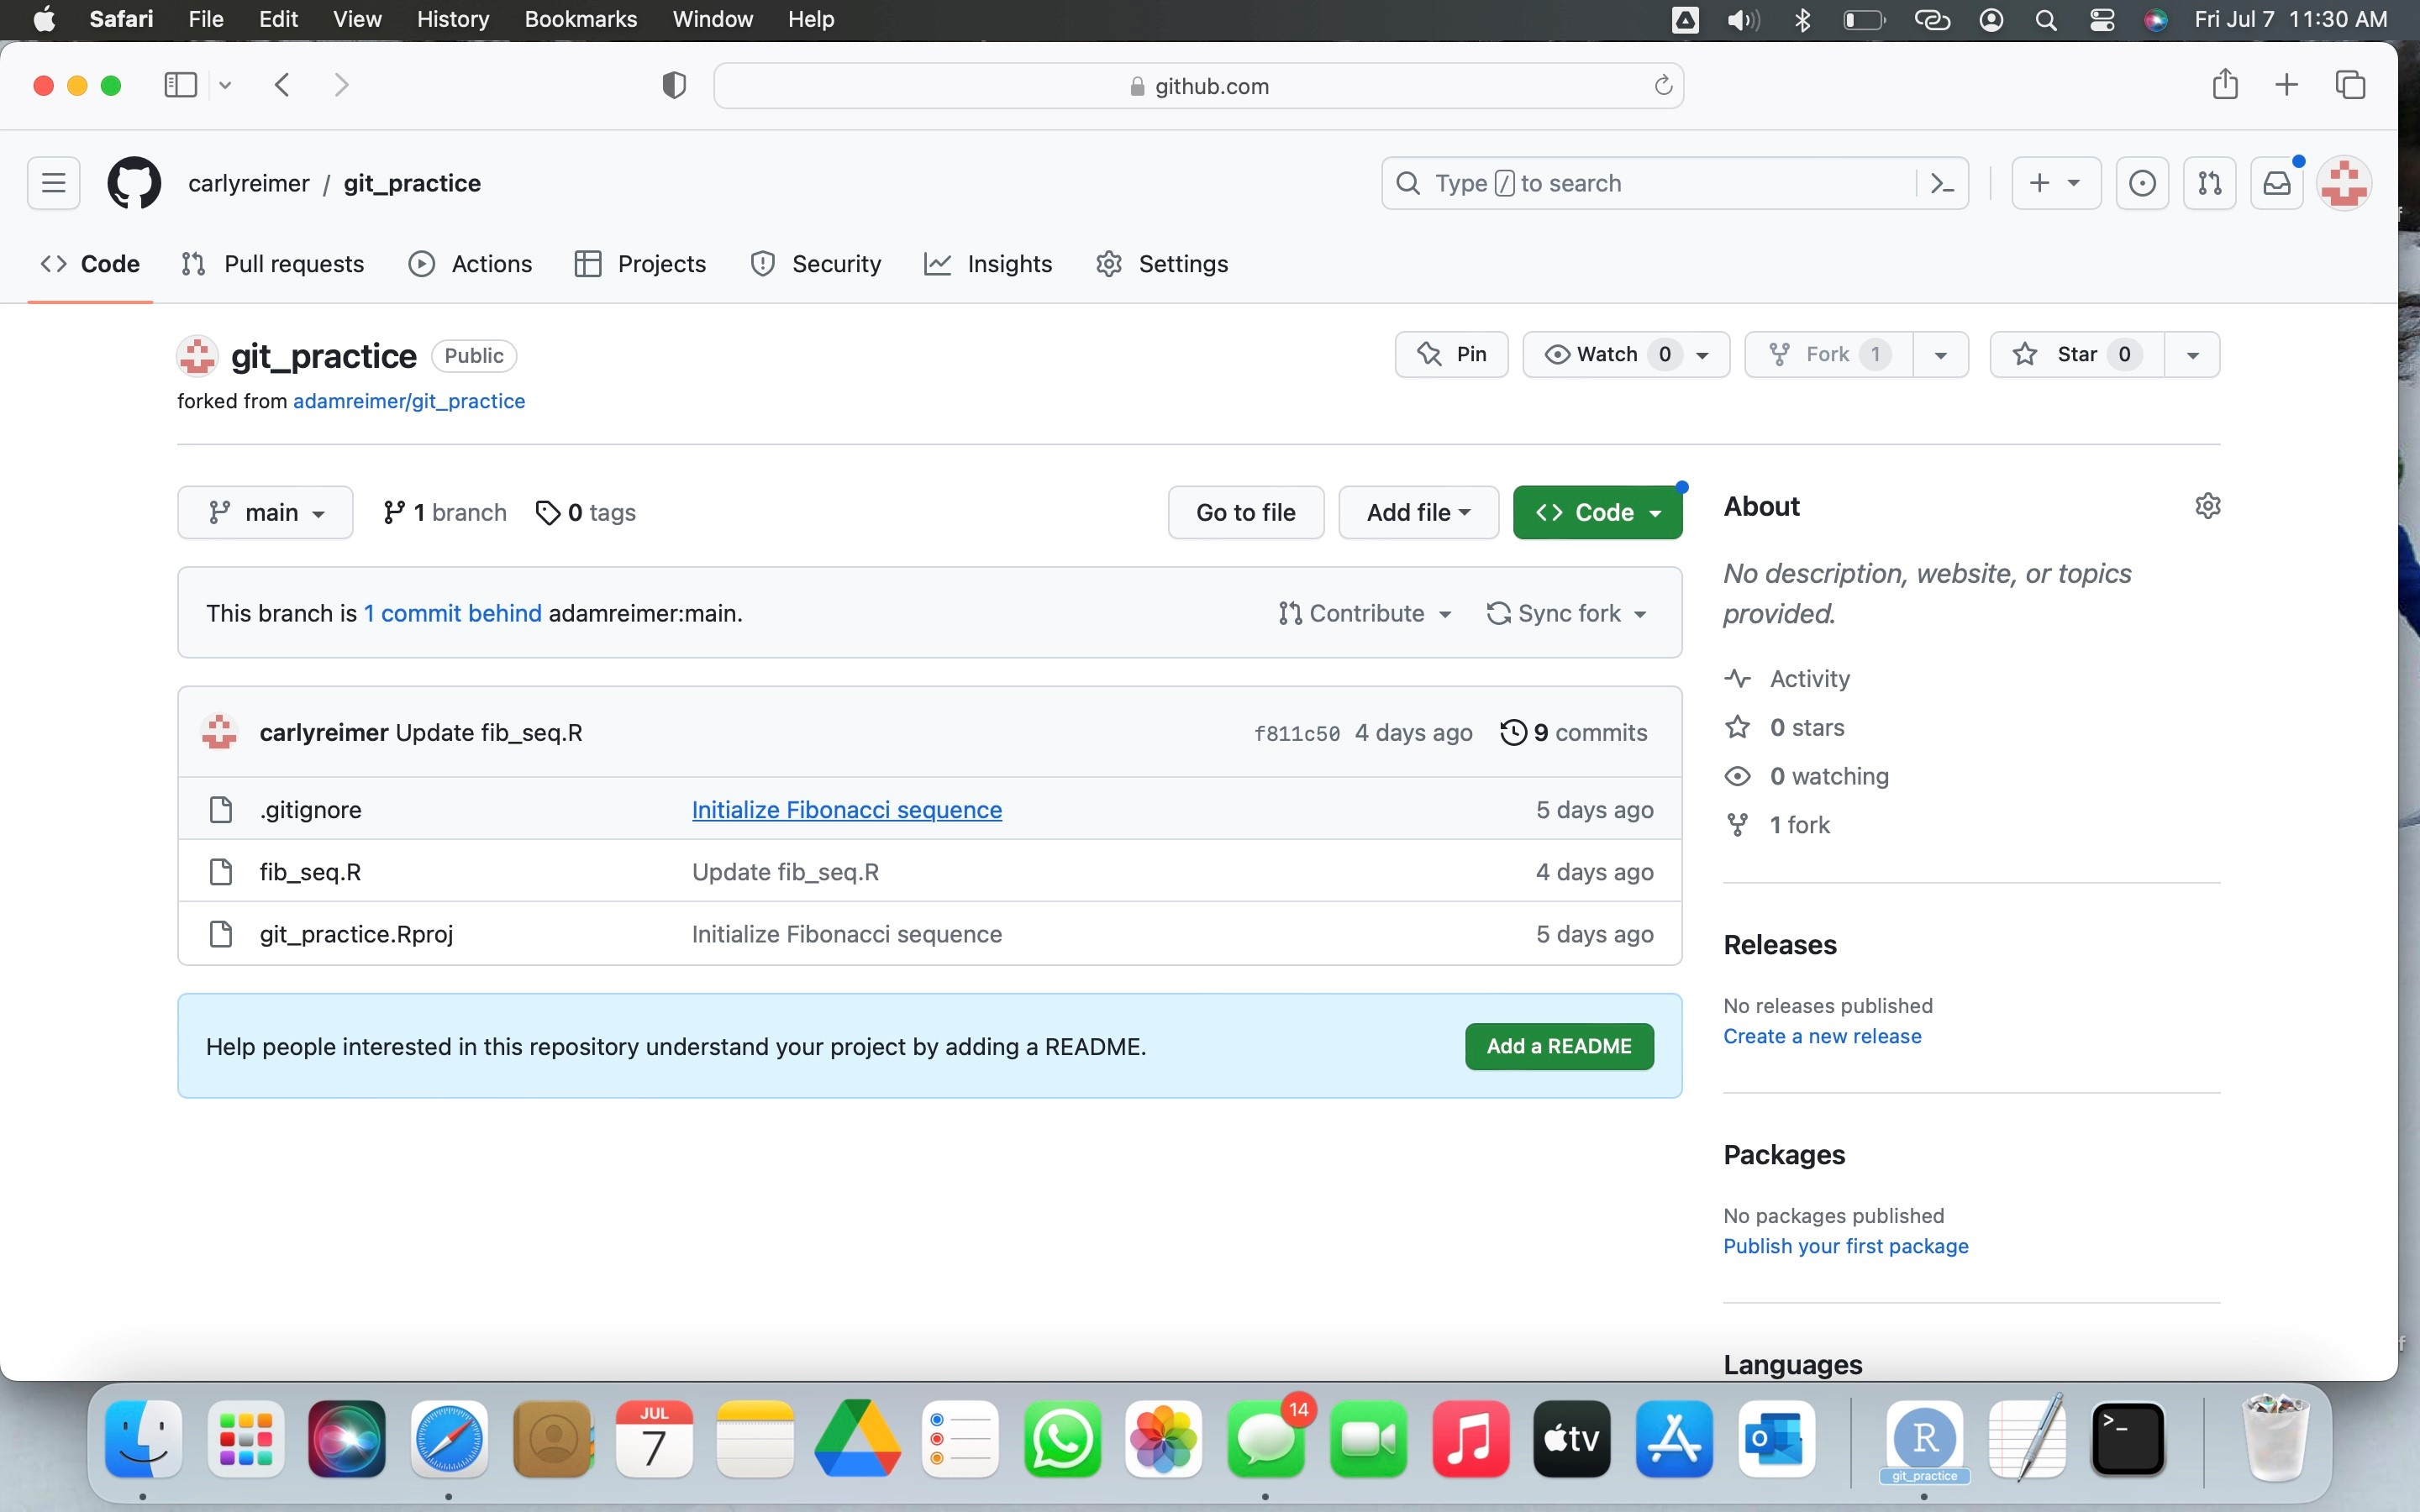
\includegraphics{forked_repository.png}

}

\caption{The forked git\_practice repository in Carly Reimer's GitHub
account}

\end{figure}

Using the same commands describe above Carly cloned the forked
repository, made changes, added the changed file, committed the changes,
and pushed the result back to her forked repository on Github. Pull
requests are so named because Carly is asking me to pull her forked
repository back into my original repository. The initiate a pull request
the owner of the forked repository (Carly) navigates to the original
repository and presses the \emph{Pull request} button. The pull request
looked like this when veiwed from my account:

\begin{figure}

{\centering 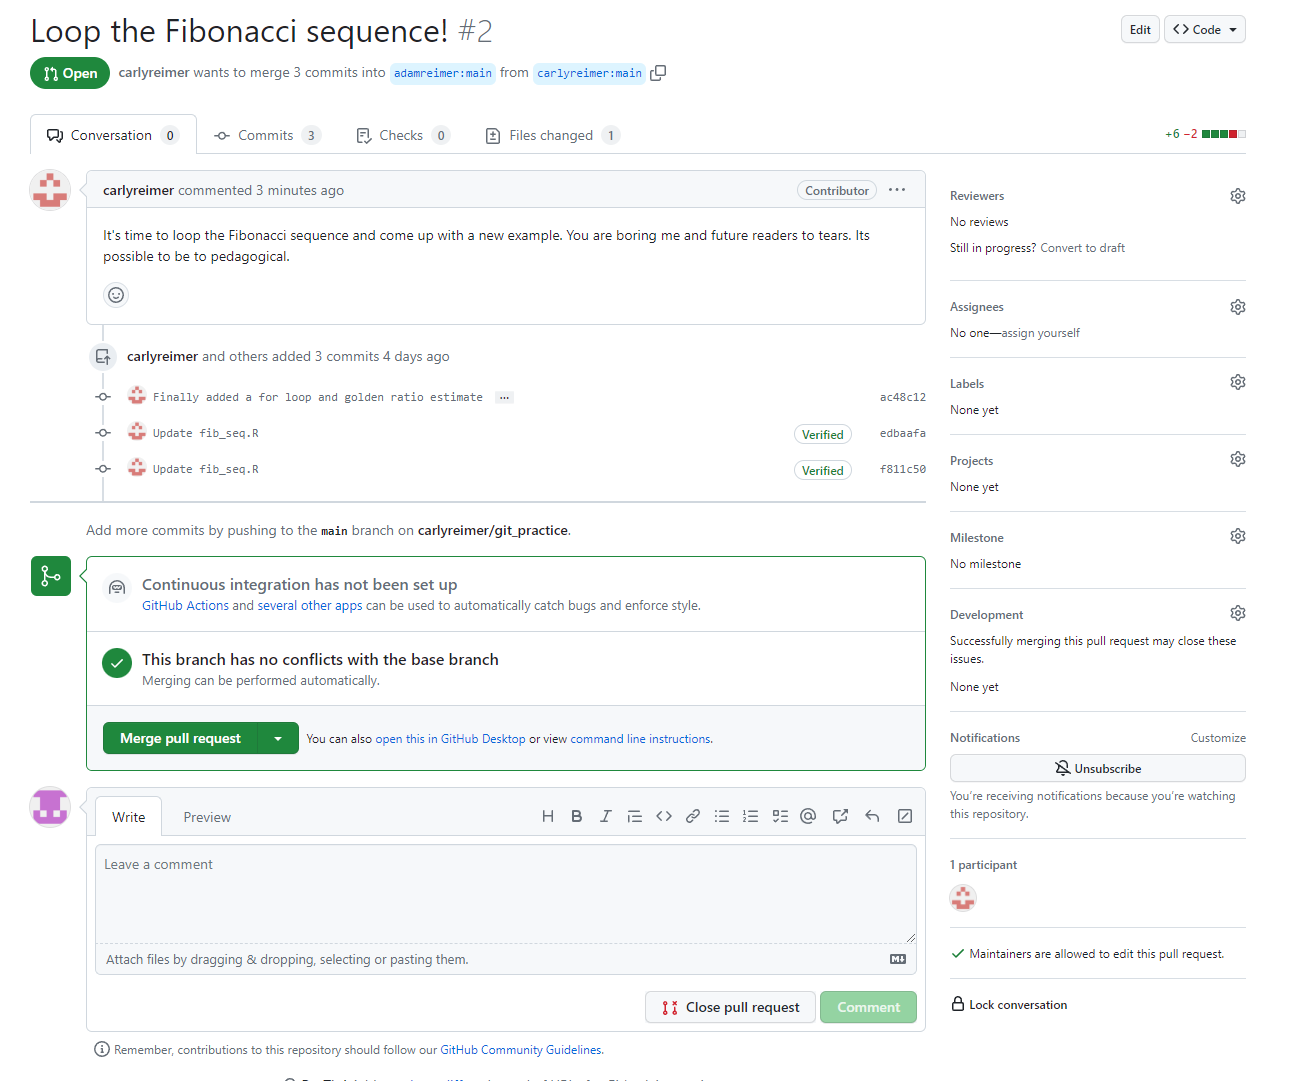
\includegraphics{pull_request_AR.PNG}

}

\caption{The pull request summary screen.}

\end{figure}

Navigating the the \emph{Files changed} button allows the repository
owner to review line by line changes associated with the pull request.
In this case, I deemed the suggestions reasonable and accepted them
without comment but there are capabilities to comments and modify the
changes before they are accepted.

\begin{figure}

{\centering 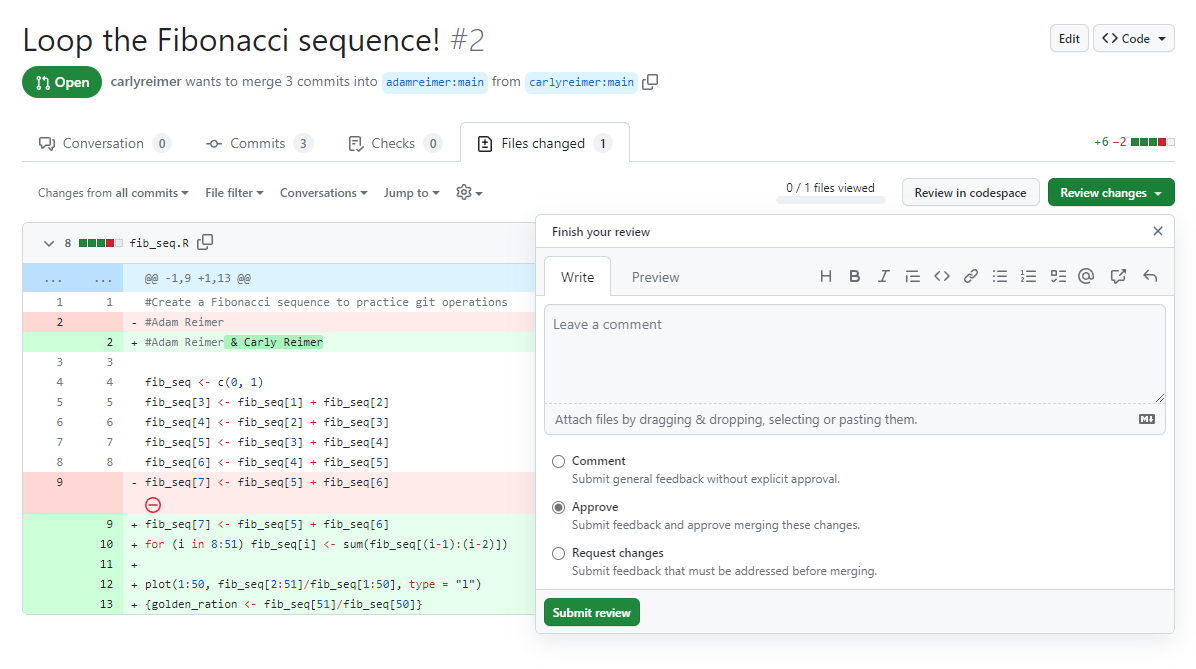
\includegraphics{pull_request_AR_approve.PNG}

}

\caption{The pull request review/approval screen}

\end{figure}

After the request is approved the original owner can merge the pull
request from within GitHub.

\begin{figure}

{\centering 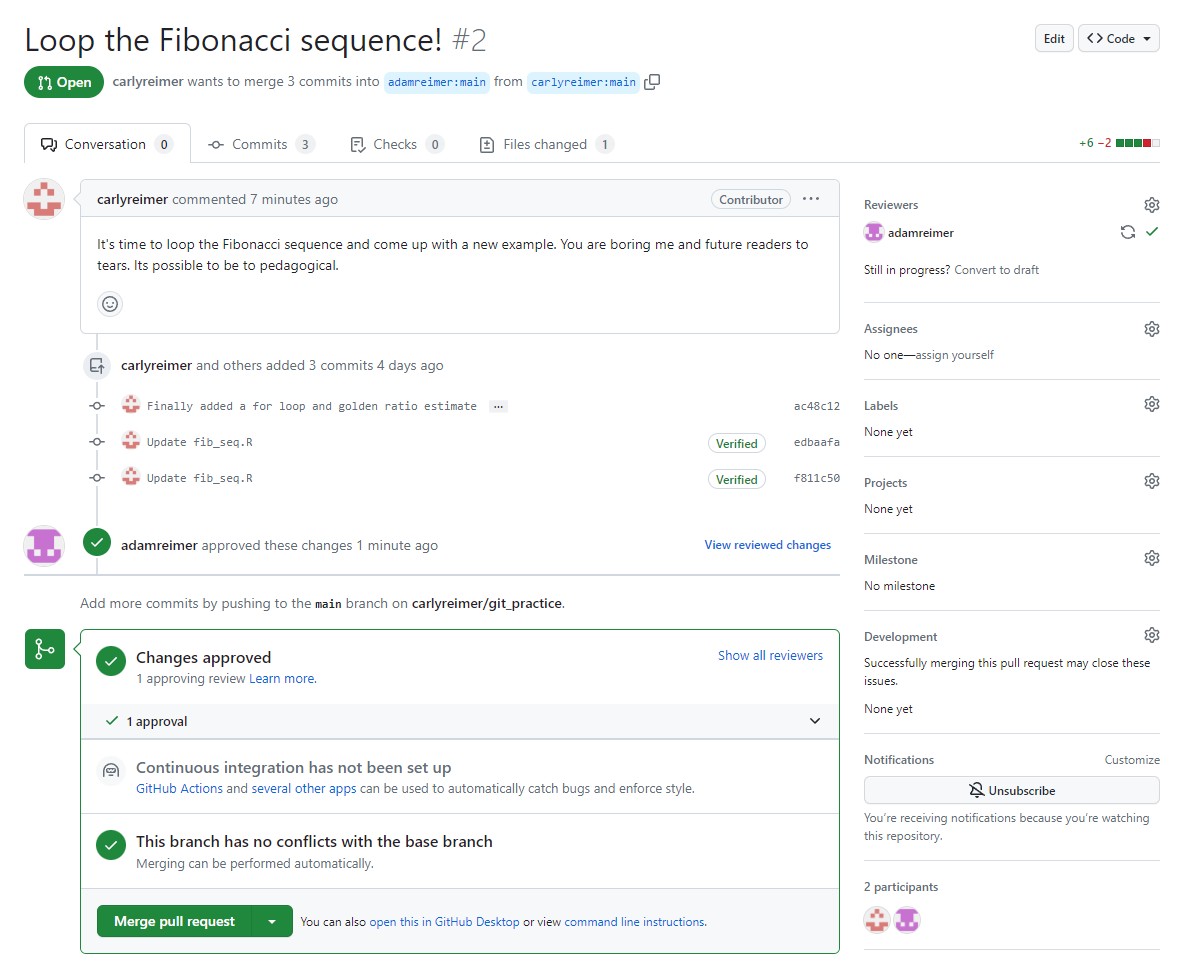
\includegraphics{pull_request_AR_merge.PNG}

}

\caption{Merging a pull request}

\end{figure}

After merging the pull request; Carly's local repository, the forked
repository, and the original remote repository are synced while Adam's
local repository is behind. This situation could be fixed with
\texttt{git\ pull}.

\begin{Shaded}
\begin{Highlighting}[]
\NormalTok{amreimer@DFGSXQDSF206801 MINGW64 /s/RTS/Reimer/Research\_Best\_Practices/git\_practice (main)}
\NormalTok{$ git pull}
\NormalTok{remote: Enumerating objects: 12, done.}
\NormalTok{remote: Counting objects: 100\% (12/12), done.}
\NormalTok{remote: Compressing objects: 100\% (7/7), done.}
\NormalTok{remote: Total 10 (delta 3), reused 9 (delta 3), pack{-}reused 0}
\NormalTok{Unpacking objects: 100\% (10/10), 2.60 KiB | 1024 bytes/s, done.}
\NormalTok{From https://github.com/adamreimer/git\_practice}
\NormalTok{   f732cdb..22dcfea  main       {-}\textgreater{} origin/main}
\NormalTok{Updating f732cdb..22dcfea}
\NormalTok{Fast{-}forward}
\NormalTok{ fib\_seq.R | 8 ++++++{-}{-}}
\NormalTok{ 1 file changed, 6 insertions(+), 2 deletions({-})}
\end{Highlighting}
\end{Shaded}

\bookmarksetup{startatroot}

\hypertarget{intermediate-git-workflow}{%
\chapter{Intermediate Git Workflow}\label{intermediate-git-workflow}}

The intermediate Git workflow introduces a new concept: branches.
Efficient use of branches and a well thought out branching strategy will
aid the analyst in Git use and is also a powerful tool for model
development.

\hypertarget{branches-and-branch-strategy}{%
\subsection{Branches and Branch
strategy}\label{branches-and-branch-strategy}}

In Git a branch is a pointer to a specific commit or set of commits
which allow you to separate model development tasks into smaller
subunits. I learned branching from
\href{https://nvie.com/posts/a-successful-git-branching-model/}{this
guy} and in what follows I simplify his workflow into something that
works well for complicated fisheries analyses. Let's start by creating a
new branch named \texttt{develop} using the command
\texttt{git\ checkout}. The argument \texttt{-b} tells Git to checkout a
new branch while the arguments \texttt{develop} and \texttt{main} tell
Git the name of the new branch and that the new branch should branch
from the \texttt{main} branch.

\begin{Shaded}
\begin{Highlighting}[]
\NormalTok{amreimer@DFGSXQDSF206801 MINGW64 /s/RTS/Reimer/Research\_Best\_Practices/git\_practice (main)}
\NormalTok{$ git checkout {-}b develop main}
\NormalTok{Switched to a new branch \textquotesingle{}develop\textquotesingle{}}
\end{Highlighting}
\end{Shaded}

The core concept in the Git Flow branching strategy is to always have
two active branches; \texttt{main} and \texttt{develop}. The
\texttt{main} branch is stable in that you make limited commits to it
and those commits are associated with internal or external reporting
including FDS reports, BOF memos, or conference presentations. Because
the \texttt{main} branch will largely be static interested collaborators
can quickly identify the analysis at the time periods where the analysis
was reported.

The \texttt{develop} branch is the working branch and will have frequent
commits relative to analysis progress. The \texttt{develop} branch
merges into \texttt{main} at reporting periods and is the branched from
whenever a new feature is being developed.

Feature branches are created frequently as new features are envisioned
and developed. A best practice is to create a new feature branch, with a
descriptive name, every time your create a new feature. When the feature
is completed it is merged back into develop, left as a record without a
merge, or deleted. In my work, feature branches are mostly merged back
into develop, and this occurs whenever I create a feature which improves
the analysis. Feature branches are left unmerged when I want to retain a
record of having tried something (and the result) but do not think it
improves the overall analysis. Feature branches are deleted without
merging when something just did not work out and is also not worth
retaining as a record. Notice that liberal use of feature branches keep
the \texttt{main} and \texttt{develop} branches clean and can isolate
those two primary branches of a lot of the sloppiness that is a
byproduct of actively engaging in the scientific process.

Let's practice Git Flow. In the terminal session which follows we create
a new branch called \texttt{cleanup} with \texttt{git\ checkout}, modify
the file \texttt{fib\_seq.R} by deleting several lines, show the changes
using \texttt{git\ diff}, add those changes, and commit those changes.

\begin{Shaded}
\begin{Highlighting}[]
\NormalTok{amreimer@DFGSXQDSF206801 MINGW64 /s/RTS/Reimer/Research\_Best\_Practices/git\_practice (develop)}
\NormalTok{$ git checkout {-}b cleanup develop}
\NormalTok{Switched to a new branch \textquotesingle{}cleanup\textquotesingle{}}

\NormalTok{amreimer@DFGSXQDSF206801 MINGW64 /s/RTS/Reimer/Research\_Best\_Practices/git\_practice (cleanup)}
\NormalTok{$ git status}
\NormalTok{On branch cleanup}
\NormalTok{Changes not staged for commit:}
\NormalTok{  (use "git add \textless{}file\textgreater{}..." to update what will be committed)}
\NormalTok{  (use "git restore \textless{}file\textgreater{}..." to discard changes in working directory)}
\NormalTok{        modified:   fib\_seq.R}

\NormalTok{no changes added to commit (use "git add" and/or "git commit {-}a")}

\NormalTok{amreimer@DFGSXQDSF206801 MINGW64 /s/RTS/Reimer/Research\_Best\_Practices/git\_practice (cleanup)}
\NormalTok{$ git diff}
\NormalTok{diff {-}{-}git a/fib\_seq.R b/fib\_seq.R}
\NormalTok{index 984a0a5..97be5b3 100644}
\NormalTok{{-}{-}{-} a/fib\_seq.R}
\NormalTok{+++ b/fib\_seq.R}
\NormalTok{@@ {-}2,12 +2,7 @@}
\NormalTok{ \#Adam Reimer \& Carly Reimer}

\NormalTok{ fib\_seq \textless{}{-} c(0, 1)}
\NormalTok{{-}fib\_seq[3] \textless{}{-} fib\_seq[1] + fib\_seq[2]}
\NormalTok{{-}fib\_seq[4] \textless{}{-} fib\_seq[2] + fib\_seq[3]}
\NormalTok{{-}fib\_seq[5] \textless{}{-} fib\_seq[3] + fib\_seq[4]}
\NormalTok{{-}fib\_seq[6] \textless{}{-} fib\_seq[4] + fib\_seq[5]}
\NormalTok{{-}fib\_seq[7] \textless{}{-} fib\_seq[5] + fib\_seq[6]}
\NormalTok{{-}for (i in 8:51) fib\_seq[i] \textless{}{-} sum(fib\_seq[(i{-}1):(i{-}2)])}
\NormalTok{+for (i in 3:51) fib\_seq[i] \textless{}{-} sum(fib\_seq[(i{-}1):(i{-}2)])}

\NormalTok{ plot(1:50, fib\_seq[2:51]/fib\_seq[1:50], type = "l")}
\NormalTok{{-}\{golden\_ration \textless{}{-} fib\_seq[51]/fib\_seq[50]\}}
\NormalTok{+\{golden\_ratio \textless{}{-} fib\_seq[51]/fib\_seq[50]\}}

\NormalTok{amreimer@DFGSXQDSF206801 MINGW64 /s/RTS/Reimer/Research\_Best\_Practices/git\_practice (cleanup)}
\NormalTok{$ git add fib\_seq.R}

\NormalTok{amreimer@DFGSXQDSF206801 MINGW64 /s/RTS/Reimer/Research\_Best\_Practices/git\_practice (cleanup)}
\NormalTok{$ git commit {-}m "remove maanual Fibonacci calculations" {-}m "manual calculations become redundent now that we are using recurstion to get the series."}
\NormalTok{[cleanup 8b28369] remove maanual Fibonacci calculations}
\NormalTok{ 1 file changed, 2 insertions(+), 7 deletions({-})}

\NormalTok{amreimer@DFGSXQDSF206801 MINGW64 /s/RTS/Reimer/Research\_Best\_Practices/git\_practice (develop)}
\NormalTok{$}
\end{Highlighting}
\end{Shaded}

\hypertarget{git-merge}{%
\subsection{git merge}\label{git-merge}}

The changes above are reasonable and the new feature tried on the
\texttt{cleanup} branch is useful. In the terminal session below we use
\texttt{git\ checkout} to switch back to the \texttt{develop} branch,
\texttt{git\ merge} to merge the \texttt{cleanup} branch with the
\texttt{develop} branch, and \texttt{git\ branch} to delete the
\texttt{cleanup} branch now that it's change has been incorporated into
\texttt{develop}.

\begin{Shaded}
\begin{Highlighting}[]
\NormalTok{amreimer@DFGSXQDSF206801 MINGW64 /s/RTS/Reimer/Research\_Best\_Practices/git\_practice (cleanup)}
\NormalTok{$ git checkout develop}
\NormalTok{Switched to branch \textquotesingle{}develop\textquotesingle{}}

\NormalTok{amreimer@DFGSXQDSF206801 MINGW64 /s/RTS/Reimer/Research\_Best\_Practices/git\_practice (develop)}
\NormalTok{$ git merge {-}{-}no{-}ff cleanup}
\NormalTok{Merge made by the \textquotesingle{}ort\textquotesingle{} strategy.}
\NormalTok{ fib\_seq.R | 9 ++{-}{-}{-}{-}{-}{-}{-}}
\NormalTok{ 1 file changed, 2 insertions(+), 7 deletions({-})}

\NormalTok{amreimer@DFGSXQDSF206801 MINGW64 /s/RTS/Reimer/Research\_Best\_Practices/git\_practice (develop)}
\NormalTok{$ git branch {-}d cleanup}
\NormalTok{Deleted branch cleanup (was 8b28369).}

\NormalTok{amreimer@DFGSXQDSF206801 MINGW64 /s/RTS/Reimer/Research\_Best\_Practices/git\_practice (develop)}
\NormalTok{$}
\end{Highlighting}
\end{Shaded}

\hypertarget{merge-conflicts}{%
\subsubsection{Merge conflicts}\label{merge-conflicts}}

Merge conflicts can occur any time we are merging two branches. In what
follows we will intentionally create a merge conflict and fix it. In the
terminal session below I create a new branch named \texttt{label\_plot},
and while working on that branch modify the file \texttt{fib\_seq.R} by
adding informative figure labels and then stage/commit those changes.

\begin{Shaded}
\begin{Highlighting}[]
\NormalTok{amreimer@DFGSXQDSF206801 MINGW64 /s/RTS/Reimer/Research\_Best\_Practices/git\_practice (develop)}
\NormalTok{$ git checkout {-}b label\_plot develop}
\NormalTok{Switched to a new branch \textquotesingle{}label\_plot\textquotesingle{}}

\NormalTok{amreimer@DFGSXQDSF206801 MINGW64 /s/RTS/Reimer/Research\_Best\_Practices/git\_practice (label\_plot)}
\NormalTok{$ git status}
\NormalTok{On branch label\_plot}
\NormalTok{Changes not staged for commit:}
\NormalTok{  (use "git add \textless{}file\textgreater{}..." to update what will be committed)}
\NormalTok{  (use "git restore \textless{}file\textgreater{}..." to discard changes in working directory)}
\NormalTok{        modified:   fib\_seq.R}

\NormalTok{no changes added to commit (use "git add" and/or "git commit {-}a")}

\NormalTok{amreimer@DFGSXQDSF206801 MINGW64 /s/RTS/Reimer/Research\_Best\_Practices/git\_practice (label\_plot)}
\NormalTok{$ git add fib\_seq.R}

\NormalTok{amreimer@DFGSXQDSF206801 MINGW64 /s/RTS/Reimer/Research\_Best\_Practices/git\_practice (label\_plot)}
\NormalTok{$ git commit {-}m "Added axis labels to golden ratio plot." {-}m "Not a lot to say but hammering home the idea that more informative messages are better. In this case I added labels to demonstrate a merge conflict. Will add different labels to the same file/figure on branch develop to create the conflict."}
\NormalTok{[label\_plot a4c0f61] Added axis labels to golden ratio plot.}
\NormalTok{ 1 file changed, 4 insertions(+), 1 deletion({-})}
 
\NormalTok{amreimer@DFGSXQDSF206801 MINGW64 /s/RTS/Reimer/Research\_Best\_Practices/git\_practice (label\_plot)}
\NormalTok{$}
\end{Highlighting}
\end{Shaded}

A merge into the \texttt{develop} branch at this stage would be both
appropriate and successful. The new feature was added to the feature
branch \texttt{label\_plot} was a improvement, and the \texttt{develop}
branch is unchanged. Instead we will intentionally change the develop
branch (violating the spirit of Git Flow) to demonstrate a merge
conflict. In the terminal session that follows we: checkout the
\texttt{develop} branch and while working on that branch modified the
file \texttt{fib\_seq.R} by adding less informative figure labels, and
stage/commit those changes. We then use \texttt{git\ show} to look at
the copy of \texttt{fib\_seq.R} from both the \texttt{develop} and
\texttt{label\_plot} branches. Notice that the axis labels from the
\texttt{label\_plot} branch are more informative. Because the values
given to the \texttt{xlab} and \texttt{ylab} arguments were modified in
both branches we can expect a merge conflict and, as expected, a merge
conflict results from attempting to merge these branches.

\begin{Shaded}
\begin{Highlighting}[]
\NormalTok{amreimer@DFGSXQDSF206801 MINGW64 /s/RTS/Reimer/Research\_Best\_Practices/git\_practice (label\_plot)}
\NormalTok{$ git checkout develop}
\NormalTok{Switched to branch \textquotesingle{}develop\textquotesingle{}}

\NormalTok{amreimer@DFGSXQDSF206801 MINGW64 /s/RTS/Reimer/Research\_Best\_Practices/git\_practice (develop)}
\NormalTok{$ git status}
\NormalTok{On branch develop}
\NormalTok{Changes not staged for commit:}
\NormalTok{  (use "git add \textless{}file\textgreater{}..." to update what will be committed)}
\NormalTok{  (use "git restore \textless{}file\textgreater{}..." to discard changes in working directory)}
\NormalTok{        modified:   fib\_seq.R}

\NormalTok{no changes added to commit (use "git add" and/or "git commit {-}a")}

\NormalTok{amreimer@DFGSXQDSF206801 MINGW64 /s/RTS/Reimer/Research\_Best\_Practices/git\_practice (develop)}
\NormalTok{$ git add fib\_seq.R}

\NormalTok{amreimer@DFGSXQDSF206801 MINGW64 /s/RTS/Reimer/Research\_Best\_Practices/git\_practice (develop)}
\NormalTok{$ git commit {-}m "Added labels to the golden ratio figure" {-}m "These labels are intentionally less informative that the labels added on the feature branch to demonstrate that feature branches are where you do the work which you then merge into develop."}
\NormalTok{[develop d0d260e] Added labels to the golden ratio figure}
\NormalTok{ 1 file changed, 4 insertions(+), 1 deletion({-})}

\NormalTok{amreimer@DFGSXQDSF206801 MINGW64 /s/RTS/Reimer/Research\_Best\_Practices/git\_practice (develop)}
\NormalTok{$ git show develop:fib\_seq.R}
\NormalTok{\#Create a Fibonacci sequence to practice git operations}
\NormalTok{\#Adam Reimer \& Carly Reimer}

\NormalTok{fib\_seq \textless{}{-} c(0, 1)}
\NormalTok{for (i in 3:51) fib\_seq[i] \textless{}{-} sum(fib\_seq[(i{-}1):(i{-}2)])}

\NormalTok{plot(1:50, fib\_seq[2:51]/fib\_seq[1:50],}
\NormalTok{     type = "l",}
\NormalTok{     xlab = "Number",}
\NormalTok{     ylab = "Ratio")}
\NormalTok{\{golden\_ratio \textless{}{-} fib\_seq[51]/fib\_seq[50]\}}

\NormalTok{amreimer@DFGSXQDSF206801 MINGW64 /s/RTS/Reimer/Research\_Best\_Practices/git\_practice (develop)}
\NormalTok{$ git show label\_plot:fib\_seq.R}
\NormalTok{\#Create a Fibonacci sequence to practice git operations}
\NormalTok{\#Adam Reimer \& Carly Reimer}

\NormalTok{fib\_seq \textless{}{-} c(0, 1)}
\NormalTok{for (i in 3:51) fib\_seq[i] \textless{}{-} sum(fib\_seq[(i{-}1):(i{-}2)])}

\NormalTok{plot(1:50, fib\_seq[2:51]/fib\_seq[1:50],}
\NormalTok{     type = "l",}
\NormalTok{     xlab = "Fibonacci Number in Denominator",}
\NormalTok{     ylab = "Ratio Between Succesive Fibonacci Numbers")}
\NormalTok{\{golden\_ratio \textless{}{-} fib\_seq[51]/fib\_seq[50]\}}

\NormalTok{amreimer@DFGSXQDSF206801 MINGW64 /s/RTS/Reimer/Research\_Best\_Practices/git\_practice (develop)}
\NormalTok{$ git merge {-}{-}no{-}ff label\_plot}
\NormalTok{Auto{-}merging fib\_seq.R}
\NormalTok{CONFLICT (content): Merge conflict in fib\_seq.R}
\NormalTok{Automatic merge failed; fix conflicts and then commit the result.}

\NormalTok{amreimer@DFGSXQDSF206801 MINGW64 /s/RTS/Reimer/Research\_Best\_Practices/git\_practice (develop)}
\NormalTok{$}
\end{Highlighting}
\end{Shaded}

When there is a merge conflict Git modifies the file being merged to
help the user decide how to proceed. Git adds
\texttt{\textless{}\textless{}\textless{}\textless{}\textless{}\textless{}\textless{}\ HEAD}
above the merge conflict. The text \texttt{======} separates the merge
conflict into code derived from each branch. Code between
\texttt{\textless{}\textless{}\textless{}\textless{}\textless{}\textless{}\ HEAD}
and \texttt{======} indicates code which was present in the branch being
merged into (\texttt{develop} in this case) while code between
\texttt{======} and
\texttt{\textgreater{}\textgreater{}\textgreater{}\textgreater{}\textgreater{}\textgreater{}\ label\_plot}
indicates code which was present in the branch being merged
(\texttt{label\_plot} in this case). I've shown what that
\texttt{fib\_seq.R} file in my working directory looks like using the
terminal command \texttt{cat,} but that is only for demonstrative
purposes. Normally, I would just open the file in RStudio, and it would
look exactly the same. To proceed the user has to decide which code to
keep, save the modified file, and stage/commit the changes. For this
example I deleted everything between
\texttt{\textless{}\textless{}\textless{}\textless{}\textless{}\textless{}\ HEAD}
and \texttt{======} inclusive as well as the line
\texttt{\textgreater{}\textgreater{}\textgreater{}\textgreater{}\textgreater{}\textgreater{}\ label\_plot}.
These deletions made the file \texttt{fib\_seq.R} we merged match the
version in the \texttt{label\_plot} branch.

\begin{Shaded}
\begin{Highlighting}[]
\NormalTok{amreimer@DFGSXQDSF206801 MINGW64 /s/RTS/Reimer/Research\_Best\_Practices/git\_practice (develop|MERGING)}
\NormalTok{$ cat fib\_seq.R}
\NormalTok{\#Create a Fibonacci sequence to practice git operations}
\NormalTok{\#Adam Reimer \& Carly Reimer}

\NormalTok{fib\_seq \textless{}{-} c(0, 1)}
\NormalTok{for (i in 3:51) fib\_seq[i] \textless{}{-} sum(fib\_seq[(i{-}1):(i{-}2)])}

\NormalTok{plot(1:50, fib\_seq[2:51]/fib\_seq[1:50],}
\NormalTok{\textless{}\textless{}\textless{}\textless{}\textless{}\textless{} HEAD}
\NormalTok{     type = "l",}
\NormalTok{     xlab = "Number",}
\NormalTok{     ylab = "Ratio")}
\NormalTok{======}
\NormalTok{     type = "l",}
\NormalTok{     xlab = "Fibonacci Number in Denominator",}
\NormalTok{     ylab = "Ratio Between Succesive Fibonacci Numbers")}
\NormalTok{\textgreater{}\textgreater{}\textgreater{}\textgreater{}\textgreater{}\textgreater{} label\_plot}
\NormalTok{\{golden\_ratio \textless{}{-} fib\_seq[51]/fib\_seq[50]\}}

\NormalTok{amreimer@DFGSXQDSF206801 MINGW64 /s/RTS/Reimer/Research\_Best\_Practices/git\_practice (develop|MERGING)}
\NormalTok{$ git status}
\NormalTok{On branch develop}
\NormalTok{You have unmerged paths.}
\NormalTok{  (fix conflicts and run "git commit")}
\NormalTok{  (use "git merge {-}{-}abort" to abort the merge)}

\NormalTok{Unmerged paths:}
\NormalTok{  (use "git add \textless{}file\textgreater{}..." to mark resolution)}
\NormalTok{        both modified:   fib\_seq.R}

\NormalTok{no changes added to commit (use "git add" and/or "git commit {-}a")}

\NormalTok{amreimer@DFGSXQDSF206801 MINGW64 /s/RTS/Reimer/Research\_Best\_Practices/git\_practice (develop|MERGING)}
\NormalTok{$ git add fib\_seq.R}

\NormalTok{amreimer@DFGSXQDSF206801 MINGW64 /s/RTS/Reimer/Research\_Best\_Practices/git\_practice (develop|MERGING)}
\NormalTok{$ git commit {-}m "fixed merge conflict by accepting changes from label\_plot branch" {-}m "Mmaybe the only good example of a situation were a description is not nessesary."}
\NormalTok{[develop ad2149a] fixed merge conflict by accepting changes from label\_plot branch}

\NormalTok{amreimer@DFGSXQDSF206801 MINGW64 /s/RTS/Reimer/Research\_Best\_Practices/git\_practice (develop)}
\NormalTok{$ git status}
\NormalTok{On branch develop}
\NormalTok{nothing to commit, working tree clean}

\NormalTok{amreimer@DFGSXQDSF206801 MINGW64 /s/RTS/Reimer/Research\_Best\_Practices/git\_practice (develop)}
\NormalTok{$}
\end{Highlighting}
\end{Shaded}

\hypertarget{interacting-with-your-git-history}{%
\subsection{Interacting with your Git
history}\label{interacting-with-your-git-history}}

\hypertarget{restoring-a-previous-version-of-a-file}{%
\subsubsection{Restoring a previous version of a
file}\label{restoring-a-previous-version-of-a-file}}

You can also use \texttt{git\ checkout} to recall a single file from a
previous commit. In the terminal sequence below I use \texttt{cat} and
\texttt{git\ show} to show that the file in my work directory and the
file in the most recent commit to the \texttt{develop} branch are the
same file. Notice a call to \texttt{git\ status} reports the same thing
without showing the files explicitly.

\begin{Shaded}
\begin{Highlighting}[]
\NormalTok{amreimer@DFGSXQDSF206801 MINGW64 /s/RTS/Reimer/Research\_Best\_Practices/git\_practice (develop)}
\NormalTok{$ cat fib\_seq.R}
\NormalTok{\#Create a Fibonacci sequence to practice git operations}
\NormalTok{\#Adam Reimer \& Carly Reimer}

\NormalTok{fib\_seq \textless{}{-} c(0, 1)}
\NormalTok{for (i in 3:51) fib\_seq[i] \textless{}{-} sum(fib\_seq[(i{-}1):(i{-}2)])}

\NormalTok{plot(1:50, fib\_seq[2:51]/fib\_seq[1:50],}
\NormalTok{     type = "l",}
\NormalTok{     xlab = "Fibonacci Number in Denominator",}
\NormalTok{     ylab = "Ratio Between Succesive Fibonacci Numbers")}
\NormalTok{\{golden\_ratio \textless{}{-} fib\_seq[51]/fib\_seq[50]\}}

\NormalTok{amreimer@DFGSXQDSF206801 MINGW64 /s/RTS/Reimer/Research\_Best\_Practices/git\_practice (develop)}
\NormalTok{$ git show develop:fib\_seq.R}
\NormalTok{\#Create a Fibonacci sequence to practice git operations}
\NormalTok{\#Adam Reimer \& Carly Reimer}

\NormalTok{fib\_seq \textless{}{-} c(0, 1)}
\NormalTok{for (i in 3:51) fib\_seq[i] \textless{}{-} sum(fib\_seq[(i{-}1):(i{-}2)])}

\NormalTok{plot(1:50, fib\_seq[2:51]/fib\_seq[1:50],}
\NormalTok{     type = "l",}
\NormalTok{     xlab = "Fibonacci Number in Denominator",}
\NormalTok{     ylab = "Ratio Between Succesive Fibonacci Numbers")}
\NormalTok{\{golden\_ratio \textless{}{-} fib\_seq[51]/fib\_seq[50]\}}

\NormalTok{amreimer@DFGSXQDSF206801 MINGW64 /s/RTS/Reimer/Research\_Best\_Practices/git\_practice (develop)}
\NormalTok{$ git status}
\NormalTok{On branch develop}
\NormalTok{nothing to commit, working tree clean}
\end{Highlighting}
\end{Shaded}

To retrieve a specific file from a prior commit you have to provide
\texttt{git\ checkout} with identifying information for the commit and
the file name. You can specify the appropriate commit with a absolute or
relative reference. For an absolute reference provide the SHA \#. For a
relative reference the shorthand is HEAD\textasciitilde\# where \# is
the number of commits prior to the latest commit. In the terminal
sequence below I used checkout to retrieve a copy of \texttt{fib\_seq.R}
from 1 commit earlier (recall this commit had the less informative x and
y axis labels). Notice the earlier version of \texttt{fib\_seq.R} was
present in my working directory (as shown in the output for
\texttt{cat}) but was not included in the latest commit to my repository
(as shown in the output to \texttt{git\ show}). If I wanted the earlier
version of \texttt{fib\_seq.R} to be associated with the most recent
commit to my repository I would need to commit the file. In this case I
did not want to change my repository so I used \texttt{git\ checkout} to
go back the the most recent version. I often use this sequence to recall
all or part of a code from a prior commit.

\begin{Shaded}
\begin{Highlighting}[]
\NormalTok{amreimer@DFGSXQDSF206801 MINGW64 /s/RTS/Reimer/Research\_Best\_Practices/git\_practice (develop)}
\NormalTok{$ git checkout HEAD\textasciitilde{}1 fib\_seq.R}
\NormalTok{Updated 1 path from abb8fba}

\NormalTok{amreimer@DFGSXQDSF206801 MINGW64 /s/RTS/Reimer/Research\_Best\_Practices/git\_practice (develop)}
\NormalTok{$ cat fib\_seq.R}
\NormalTok{\#Create a Fibonacci sequence to practice git operations}
\NormalTok{\#Adam Reimer \& Carly Reimer}

\NormalTok{fib\_seq \textless{}{-} c(0, 1)}
\NormalTok{for (i in 3:51) fib\_seq[i] \textless{}{-} sum(fib\_seq[(i{-}1):(i{-}2)])}

\NormalTok{plot(1:50, fib\_seq[2:51]/fib\_seq[1:50],}
\NormalTok{     type = "l",}
\NormalTok{     xlab = "Number",}
\NormalTok{     ylab = "Ratio")}
\NormalTok{\{golden\_ratio \textless{}{-} fib\_seq[51]/fib\_seq[50]\}}

\NormalTok{amreimer@DFGSXQDSF206801 MINGW64 /s/RTS/Reimer/Research\_Best\_Practices/git\_practice (develop)}
\NormalTok{$ git show develop:fib\_seq.R}
\NormalTok{\#Create a Fibonacci sequence to practice git operations}
\NormalTok{\#Adam Reimer \& Carly Reimer}

\NormalTok{fib\_seq \textless{}{-} c(0, 1)}
\NormalTok{for (i in 3:51) fib\_seq[i] \textless{}{-} sum(fib\_seq[(i{-}1):(i{-}2)])}

\NormalTok{plot(1:50, fib\_seq[2:51]/fib\_seq[1:50],}
\NormalTok{     type = "l",}
\NormalTok{     xlab = "Fibonacci Number in Denominator",}
\NormalTok{     ylab = "Ratio Between Succesive Fibonacci Numbers")}
\NormalTok{\{golden\_ratio \textless{}{-} fib\_seq[51]/fib\_seq[50]\}}

\NormalTok{amreimer@DFGSXQDSF206801 MINGW64 /s/RTS/Reimer/Research\_Best\_Practices/git\_practice (develop)}
\NormalTok{$ git status}
\NormalTok{On branch develop}
\NormalTok{Changes to be committed:}
\NormalTok{  (use "git restore {-}{-}staged \textless{}file\textgreater{}..." to unstage)}
\NormalTok{        modified:   fib\_seq.R}

\NormalTok{amreimer@DFGSXQDSF206801 MINGW64 /s/RTS/Reimer/Research\_Best\_Practices/git\_practice (develop)}
\NormalTok{$ git checkout HEAD fib\_seq.R}
\NormalTok{Updated 1 path from bd65128}

\NormalTok{amreimer@DFGSXQDSF206801 MINGW64 /s/RTS/Reimer/Research\_Best\_Practices/git\_practice (develop)}
\NormalTok{$ cat fib\_seq.R}
\NormalTok{\#Create a Fibonacci sequence to practice git operations}
\NormalTok{\#Adam Reimer \& Carly Reimer}

\NormalTok{fib\_seq \textless{}{-} c(0, 1)}
\NormalTok{for (i in 3:51) fib\_seq[i] \textless{}{-} sum(fib\_seq[(i{-}1):(i{-}2)])}

\NormalTok{plot(1:50, fib\_seq[2:51]/fib\_seq[1:50],}
\NormalTok{     type = "l",}
\NormalTok{     xlab = "Fibonacci Number in Denominator",}
\NormalTok{     ylab = "Ratio Between Succesive Fibonacci Numbers")}
\NormalTok{\{golden\_ratio \textless{}{-} fib\_seq[51]/fib\_seq[50]\}}

\NormalTok{amreimer@DFGSXQDSF206801 MINGW64 /s/RTS/Reimer/Research\_Best\_Practices/git\_practice (develop)}
\NormalTok{$}
\end{Highlighting}
\end{Shaded}

\hypertarget{retrieving-a-prior-commit}{%
\subsubsection{Retrieving a prior
commit}\label{retrieving-a-prior-commit}}

Yet another use of \texttt{git\ checkout} is to recall a previous commit
in it's entirety. Since our repository only has one file I created,
staged and committed a second file named \texttt{test.R} to demonstrate
this functionality. In the terminal sequence below I show the contents
of \texttt{test.R} and some now familiar content where I check the
status of my repository and stage/commit the new file.

\begin{Shaded}
\begin{Highlighting}[]
\NormalTok{amreimer@DFGSXQDSF206801 MINGW64 /s/RTS/Reimer/Research\_Best\_Practices/git\_practice (develop)}
\NormalTok{$ cat test.R}
\NormalTok{\#Blank file to see if we can use git checkout to retrieve an entire commit.}
\NormalTok{\#Proof would be seeing this file and the correct version of fib\_seq.R}

\NormalTok{amreimer@DFGSXQDSF206801 MINGW64 /s/RTS/Reimer/Research\_Best\_Practices/git\_practice (develop)}
\NormalTok{$ git status}
\NormalTok{On branch develop}
\NormalTok{Untracked files:}
\NormalTok{  (use "git add \textless{}file\textgreater{}..." to include in what will be committed)}
\NormalTok{        test.R}

\NormalTok{nothing added to commit but untracked files present (use "git add" to track)}

\NormalTok{amreimer@DFGSXQDSF206801 MINGW64 /s/RTS/Reimer/Research\_Best\_Practices/git\_practice (develop)}
\NormalTok{$ git add test.R}

\NormalTok{amreimer@DFGSXQDSF206801 MINGW64 /s/RTS/Reimer/Research\_Best\_Practices/git\_practice (develop)}
\NormalTok{$ git commit {-}m "Test.R file added. Used to test that git checkout recalls an entire commit" {-}m "added a second file so to verify both files come when I jump around commits."}
\NormalTok{[develop 4ef90af] Test.R file added. Used to test that git checkout recalls an entire commit}
\NormalTok{ 1 file changed, 2 insertions(+)}
\NormalTok{ create mode 100644 test.R}

\NormalTok{amreimer@DFGSXQDSF206801 MINGW64 /s/RTS/Reimer/Research\_Best\_Practices/git\_practice (develop)}
\NormalTok{$}
\end{Highlighting}
\end{Shaded}

To retrieve a prior commit you should create a new branch to house the
past commit until you decide what to do with it. While not strictly
necessary creating a new branch is stable and protects your
\texttt{develop} branch. In the terminal session below I use
\texttt{git\ checkout} to create a new branch called \texttt{old\_state}
and fill it with the snapshot of the \texttt{develop} branch from 2
commits earlier. I am expecting old state to be missing \texttt{test.R}
and have the less descriptive axis locations in the version of
\texttt{fib\_seq.R}. Two calls to \texttt{cat} confirm that my working
directory does not contain \texttt{test.R} and has the older version of
\texttt{fib\_seq.R}

\begin{Shaded}
\begin{Highlighting}[]
\NormalTok{amreimer@DFGSXQDSF206801 MINGW64 /s/RTS/Reimer/Research\_Best\_Practices/git\_practice (develop)}
\NormalTok{$ git checkout {-}b old\_state HEAD\textasciitilde{}2}
\NormalTok{Switched to a new branch \textquotesingle{}old\_state\textquotesingle{}}

\NormalTok{amreimer@DFGSXQDSF206801 MINGW64 /s/RTS/Reimer/Research\_Best\_Practices/git\_practice (old\_state)}
\NormalTok{$ cat fib\_seq.R}
\NormalTok{\#Create a Fibonacci sequence to practice git operations}
\NormalTok{\#Adam Reimer \& Carly Reimer}

\NormalTok{fib\_seq \textless{}{-} c(0, 1)}
\NormalTok{for (i in 3:51) fib\_seq[i] \textless{}{-} sum(fib\_seq[(i{-}1):(i{-}2)])}

\NormalTok{plot(1:50, fib\_seq[2:51]/fib\_seq[1:50],}
\NormalTok{     type = "l",}
\NormalTok{     xlab = "Number",}
\NormalTok{     ylab = "Ratio")}
\NormalTok{\{golden\_ratio \textless{}{-} fib\_seq[51]/fib\_seq[50]\}}

\NormalTok{amreimer@DFGSXQDSF206801 MINGW64 /s/RTS/Reimer/Research\_Best\_Practices/git\_practice (old\_state)}
\NormalTok{$ cat test.R}
\NormalTok{cat: test.R: No such file or directory}

\NormalTok{amreimer@DFGSXQDSF206801 MINGW64 /s/RTS/Reimer/Research\_Best\_Practices/git\_practice (old\_state)}
\NormalTok{$ git status}
\NormalTok{On branch old\_state}
\NormalTok{nothing to commit, working tree clean}

\NormalTok{amreimer@DFGSXQDSF206801 MINGW64 /s/RTS/Reimer/Research\_Best\_Practices/git\_practice (develop)}
\NormalTok{$}
\end{Highlighting}
\end{Shaded}

The next action depends on if you want the keep working on the prior
commit. If you do you can modify files and stage/commit the result as
appropriate prior to merging \texttt{old\_state} back into
\texttt{develop}. Since you purposely started the \texttt{old\_state}
feature branch from a prior version of \texttt{develop} the odds of a
merge conflict are high. It does mean it's a terrible idea but you
should be doing this with intention. In the terminal session below I
decided the prior commit was not an improvement on my original commit so
I moved back to the \texttt{develop} branch and deleted the
\texttt{old\_state} branch. Two calls to \texttt{cat} prove that the
original files were returned.

\begin{Shaded}
\begin{Highlighting}[]
\NormalTok{amreimer@DFGSXQDSF206801 MINGW64 /s/RTS/Reimer/Research\_Best\_Practices/git\_practice (old\_state)}
\NormalTok{$ git checkout develop}
\NormalTok{Switched to branch \textquotesingle{}develop\textquotesingle{}}

\NormalTok{amreimer@DFGSXQDSF206801 MINGW64 /s/RTS/Reimer/Research\_Best\_Practices/git\_practice (develop)}
\NormalTok{$ cat fib\_seq.R}
\NormalTok{\#Create a Fibonacci sequence to practice git operations}
\NormalTok{\#Adam Reimer \& Carly Reimer}

\NormalTok{fib\_seq \textless{}{-} c(0, 1)}
\NormalTok{for (i in 3:51) fib\_seq[i] \textless{}{-} sum(fib\_seq[(i{-}1):(i{-}2)])}

\NormalTok{plot(1:50, fib\_seq[2:51]/fib\_seq[1:50],}
\NormalTok{     type = "l",}
\NormalTok{     xlab = "Fibonacci Number in Denominator",}
\NormalTok{     ylab = "Ratio Between Succesive Fibonacci Numbers")}
\NormalTok{\{golden\_ratio \textless{}{-} fib\_seq[51]/fib\_seq[50]\}}

\NormalTok{amreimer@DFGSXQDSF206801 MINGW64 /s/RTS/Reimer/Research\_Best\_Practices/git\_practice (develop)}
\NormalTok{$ cat test.R}
\NormalTok{\#Blank file to see if we can use git checkout to retrieve an entire commit.}
\NormalTok{\#Proof would be seeing this file and the correct version of fib\_seq.R}

\NormalTok{amreimer@DFGSXQDSF206801 MINGW64 /s/RTS/Reimer/Research\_Best\_Practices/git\_practice (develop)}
\NormalTok{$ git branch {-}d old\_state}
\NormalTok{Deleted branch old\_state (was d0d260e).}

\NormalTok{amreimer@DFGSXQDSF206801 MINGW64 /s/RTS/Reimer/Research\_Best\_Practices/git\_practice (develop)}
\NormalTok{$}
\end{Highlighting}
\end{Shaded}

\hypertarget{deleatingreversing-a-commit}{%
\subsubsection{Deleating/Reversing a
commit}\label{deleatingreversing-a-commit}}

There are two ways to reverse a commit. The version you should choose
depends on if you have pushed the commit to a remote repository.

\hypertarget{deleting-a-local-commit}{%
\paragraph{Deleting a local commit}\label{deleting-a-local-commit}}

When the bad commit is local you can us \texttt{git\ reset} to delete
the commit. The commit will disappear from your history. To demonstrate
this command I modified the \texttt{fib\_seq.R} by adding an
inconsequential comment at the bottom of the file and used the
\texttt{cat} command to show the file. After adding and committing the
file a call to \texttt{git\ log} shows that the commit was recorded.

\begin{Shaded}
\begin{Highlighting}[]
\NormalTok{amreimer@DFGSXQDSF206801 MINGW64 /s/RTS/Reimer/Research\_Best\_Practices/git\_practice (develop)}
\NormalTok{$ cat fib\_seq.R}
\NormalTok{\#Create a Fibonacci sequence to practice git operations}
\NormalTok{\#Adam Reimer \& Carly Reimer}

\NormalTok{fib\_seq \textless{}{-} c(0, 1)}
\NormalTok{for (i in 3:51) fib\_seq[i] \textless{}{-} sum(fib\_seq[(i{-}1):(i{-}2)])}

\NormalTok{plot(1:50, fib\_seq[2:51]/fib\_seq[1:50],}
\NormalTok{     type = "l",}
\NormalTok{     xlab = "Fibonacci Number in Denominator",}
\NormalTok{     ylab = "Ratio Between Succesive Fibonacci Numbers")}
\NormalTok{\{golden\_ratio \textless{}{-} fib\_seq[51]/fib\_seq[50]\}}

\NormalTok{\#Useless comment to demonstrate how to delete a commit}

\NormalTok{amreimer@DFGSXQDSF206801 MINGW64 /s/RTS/Reimer/Research\_Best\_Practices/git\_practice (develop)}
\NormalTok{$ git add fib\_seq.R}

\NormalTok{amreimer@DFGSXQDSF206801 MINGW64 /s/RTS/Reimer/Research\_Best\_Practices/git\_practice (develop)}
\NormalTok{$ git commit {-}m "bad commit, plan to delete" {-}m "This commit has one change, a useless comment added to the fib\_seq.R file. Plan to reset the HEAD to delete the commit"}
\NormalTok{[develop ae2fe59] bad commit, plan to delete}
\NormalTok{ 1 file changed, 2 insertions(+)}

\NormalTok{amreimer@DFGSXQDSF206801 MINGW64 /s/RTS/Reimer/Research\_Best\_Practices/git\_practice (develop)}
\NormalTok{$ git log {-}{-}oneline}
\NormalTok{ae2fe59 (HEAD {-}\textgreater{} develop) bad commit, plan to delete}
\NormalTok{4ef90af Test.R file added. Used to test that git checkout recalls an entire commit}
\NormalTok{ad2149a fixed merge conflict by accepting changes from label\_plot branch}
\NormalTok{d0d260e Added labels to the golden ratio figure}
\NormalTok{a4c0f61 Added axis labels to golden ratio plot.}
\NormalTok{eb216a6 Merge branch \textquotesingle{}cleanup\textquotesingle{} into develop}
\NormalTok{8b28369 remove maanual Fibonacci calculations}
\NormalTok{22dcfea (origin/main, main) Merge pull request \#2 from carlyreimer/main}
\NormalTok{f811c50 Update fib\_seq.R}
\NormalTok{edbaafa Update fib\_seq.R}
\NormalTok{ac48c12 Finally added a for loop and golden ratio estimate}
\NormalTok{f732cdb Seventh Fibonacci number}
\NormalTok{9db5478 Sixth number in the Fibonacci seqence}
\NormalTok{5139049 Fifth entry in the Fibonacci sequence}
\NormalTok{0c92881 Fourth entry in the Fibonacci sequence}
\NormalTok{3bb6c98 Third entry in fib\_seq}
\NormalTok{e17181f Initialize Fibonacci sequence}
    
\NormalTok{amreimer@DFGSXQDSF206801 MINGW64 /s/RTS/Reimer/Research\_Best\_Practices/git\_practice (develop)}
\NormalTok{$    }
\end{Highlighting}
\end{Shaded}

In the terminal session below I use \texttt{git\ reset} to reset my
local repository to 1 commit prior to the most recent commit. Notice
that the comment I added to the most recent commit is no longer a part
of the \texttt{fib\_seq.R} file and that the commit
\texttt{ae2fe59d44eec001b949c3677f94f78e0c30a216} has been removed for
the repository. The important thing to note is \texttt{git\ reset}
changes the repository history. If you are working locally this is OK
but if you have already pushed the bad commit to a remote then deleting
a part of your history will cause problems for collaborators who pulled
the original history.

\begin{Shaded}
\begin{Highlighting}[]
\NormalTok{amreimer@DFGSXQDSF206801 MINGW64 /s/RTS/Reimer/Research\_Best\_Practices/git\_practice (develop)}
\NormalTok{$ git reset HEAD\textasciitilde{}1 {-}{-}hard}
\NormalTok{HEAD is now at 4ef90af Test.R file added. Used to test that git checkout recalls an entire commit}

\NormalTok{amreimer@DFGSXQDSF206801 MINGW64 /s/RTS/Reimer/Research\_Best\_Practices/git\_practice (develop)}
\NormalTok{$ cat fib\_seq.R}
\NormalTok{\#Create a Fibonacci sequence to practice git operations}
\NormalTok{\#Adam Reimer \& Carly Reimer}

\NormalTok{fib\_seq \textless{}{-} c(0, 1)}
\NormalTok{for (i in 3:51) fib\_seq[i] \textless{}{-} sum(fib\_seq[(i{-}1):(i{-}2)])}

\NormalTok{plot(1:50, fib\_seq[2:51]/fib\_seq[1:50],}
\NormalTok{     type = "l",}
\NormalTok{     xlab = "Fibonacci Number in Denominator",}
\NormalTok{     ylab = "Ratio Between Succesive Fibonacci Numbers")}
\NormalTok{\{golden\_ratio \textless{}{-} fib\_seq[51]/fib\_seq[50]\}}

\NormalTok{amreimer@DFGSXQDSF206801 MINGW64 /s/RTS/Reimer/Research\_Best\_Practices/git\_practice (develop)}
\NormalTok{$ git log {-}{-}oneline}
\NormalTok{4ef90af (HEAD {-}\textgreater{} develop) Test.R file added. Used to test that git checkout recalls an entire commit}
\NormalTok{ad2149a fixed merge conflict by accepting changes from label\_plot branch}
\NormalTok{d0d260e Added labels to the golden ratio figure}
\NormalTok{a4c0f61 Added axis labels to golden ratio plot.}
\NormalTok{eb216a6 Merge branch \textquotesingle{}cleanup\textquotesingle{} into develop}
\NormalTok{8b28369 remove maanual Fibonacci calculations}
\NormalTok{22dcfea (origin/main, main) Merge pull request \#2 from carlyreimer/main}
\NormalTok{f811c50 Update fib\_seq.R}
\NormalTok{edbaafa Update fib\_seq.R}
\NormalTok{ac48c12 Finally added a for loop and golden ratio estimate}
\NormalTok{f732cdb Seventh Fibonacci number}
\NormalTok{9db5478 Sixth number in the Fibonacci seqence}
\NormalTok{5139049 Fifth entry in the Fibonacci sequence}
\NormalTok{0c92881 Fourth entry in the Fibonacci sequence}
\NormalTok{3bb6c98 Third entry in fib\_seq}
\NormalTok{e17181f Initialize Fibonacci sequence}

\NormalTok{amreimer@DFGSXQDSF206801 MINGW64 /s/RTS/Reimer/Research\_Best\_Practices/git\_practice (develop)}
\NormalTok{$ git status}
\NormalTok{On branch develop}
\NormalTok{nothing to commit, working tree clean}

\NormalTok{amreimer@DFGSXQDSF206801 MINGW64 /s/RTS/Reimer/Research\_Best\_Practices/git\_practice (develop)}
\NormalTok{$}
\end{Highlighting}
\end{Shaded}

\hypertarget{reversing-a-localremote-commit}{%
\paragraph{Reversing a local/remote
commit}\label{reversing-a-localremote-commit}}

Because revising your history in a public repository is bad
collaboration Git has devised a solution. The \texttt{git\ revert}
command can also be used to undo a mistaken commit but it does so in a
very deliberate way\ldots{} by creating a new commit that exactly undoes
the prior commit. This method provides a stable Git history to your
collaborators. In the git session below I modified the
\texttt{fib\_seq.R} again (with an inconsequential comment) and
added/committed the change. \texttt{git\ log} shows the new commit.

\begin{Shaded}
\begin{Highlighting}[]
\NormalTok{amreimer@DFGSXQDSF206801 MINGW64 /s/RTS/Reimer/Research\_Best\_Practices/git\_practice (develop)}
\NormalTok{$ git status}
\NormalTok{On branch develop}
\NormalTok{Changes not staged for commit:}
\NormalTok{  (use "git add \textless{}file\textgreater{}..." to update what will be committed)}
\NormalTok{  (use "git restore \textless{}file\textgreater{}..." to discard changes in working directory)}
\NormalTok{        modified:   fib\_seq.R}

\NormalTok{no changes added to commit (use "git add" and/or "git commit {-}a")}

\NormalTok{amreimer@DFGSXQDSF206801 MINGW64 /s/RTS/Reimer/Research\_Best\_Practices/git\_practice (develop)}
\NormalTok{$ git add fib\_seq.R}

\NormalTok{amreimer@DFGSXQDSF206801 MINGW64 /s/RTS/Reimer/Research\_Best\_Practices/git\_practice (develop)}
\NormalTok{$ git commit {-}m "bad commit, plan to revert" {-}m "This commit has one change, a useless comment added to the fib\_seq.R file. Plan to revert the commit""}
\NormalTok{\textgreater{} "}
\NormalTok{[develop a0c849e] bad commit, plan to revert}
\NormalTok{ 1 file changed, 2 insertions(+)}

\NormalTok{amreimer@DFGSXQDSF206801 MINGW64 /s/RTS/Reimer/Research\_Best\_Practices/git\_practice (develop)}
\NormalTok{$ git log {-}{-}oneline}
\NormalTok{a0c849e (HEAD {-}\textgreater{} develop) bad commit, plan to revert}
\NormalTok{4ef90af Test.R file added. Used to test that git checkout recalls an entire commit}
\NormalTok{ad2149a fixed merge conflict by accepting changes from label\_plot branch}
\NormalTok{d0d260e Added labels to the golden ratio figure}
\NormalTok{a4c0f61 Added axis labels to golden ratio plot.}
\NormalTok{eb216a6 Merge branch \textquotesingle{}cleanup\textquotesingle{} into develop}
\NormalTok{8b28369 remove maanual Fibonacci calculations}
\NormalTok{22dcfea (origin/main, main) Merge pull request \#2 from carlyreimer/main}
\NormalTok{f811c50 Update fib\_seq.R}
\NormalTok{edbaafa Update fib\_seq.R}
\NormalTok{ac48c12 Finally added a for loop and golden ratio estimate}
\NormalTok{f732cdb Seventh Fibonacci number}
\NormalTok{9db5478 Sixth number in the Fibonacci seqence}
\NormalTok{5139049 Fifth entry in the Fibonacci sequence}
\NormalTok{0c92881 Fourth entry in the Fibonacci sequence}
\NormalTok{3bb6c98 Third entry in fib\_seq}
\NormalTok{e17181f Initialize Fibonacci sequence}

\NormalTok{amreimer@DFGSXQDSF206801 MINGW64 /s/RTS/Reimer/Research\_Best\_Practices/git\_practice (develop)}
\NormalTok{$}
\end{Highlighting}
\end{Shaded}

Using \texttt{git\ revert} I specify the short SHA id from the prior
commit. The call to \texttt{git\ log} shows that a new commit was added
with a message specifying the commit reverted the commit titled ``bad
commit, plan to revert''.

\begin{Shaded}
\begin{Highlighting}[]
\NormalTok{amreimer@DFGSXQDSF206801 MINGW64 /s/RTS/Reimer/Research\_Best\_Practices/git\_practice (develop)}
\NormalTok{$ git revert a0c849e}
\NormalTok{[develop 6466f85] Revert commit titled: "bad commit, plan to revert"}
\NormalTok{ 1 file changed, 2 deletions({-})}

\NormalTok{amreimer@DFGSXQDSF206801 MINGW64 /s/RTS/Reimer/Research\_Best\_Practices/git\_practice (develop)}
\NormalTok{$ git log {-}{-}oneline}
\NormalTok{6466f85 (HEAD {-}\textgreater{} develop) Revert commit titled: "bad commit, plan to revert"}
\NormalTok{a0c849e bad commit, plan to revert}
\NormalTok{4ef90af Test.R file added. Used to test that git checkout recalls an entire commit}
\NormalTok{ad2149a fixed merge conflict by accepting changes from label\_plot branch}
\NormalTok{d0d260e Added labels to the golden ratio figure}
\NormalTok{a4c0f61 Added axis labels to golden ratio plot.}
\NormalTok{eb216a6 Merge branch \textquotesingle{}cleanup\textquotesingle{} into develop}
\NormalTok{8b28369 remove maanual Fibonacci calculations}
\NormalTok{22dcfea (origin/main, main) Merge pull request \#2 from carlyreimer/main}
\NormalTok{f811c50 Update fib\_seq.R}
\NormalTok{edbaafa Update fib\_seq.R}
\NormalTok{ac48c12 Finally added a for loop and golden ratio estimate}
\NormalTok{f732cdb Seventh Fibonacci number}
\NormalTok{9db5478 Sixth number in the Fibonacci seqence}
\NormalTok{5139049 Fifth entry in the Fibonacci sequence}
\NormalTok{0c92881 Fourth entry in the Fibonacci sequence}
\NormalTok{3bb6c98 Third entry in fib\_seq}
\NormalTok{e17181f Initialize Fibonacci sequence}

\NormalTok{amreimer@DFGSXQDSF206801 MINGW64 /s/RTS/Reimer/Research\_Best\_Practices/git\_practice (develop)}
\NormalTok{$ git status}
\NormalTok{On branch develop}
\NormalTok{nothing to commit, working tree clean}

\NormalTok{amreimer@DFGSXQDSF206801 MINGW64 /s/RTS/Reimer/Research\_Best\_Practices/git\_practice (develop)}
\NormalTok{$}
\end{Highlighting}
\end{Shaded}

\hypertarget{before-you-go}{%
\subsection{Before you go!}\label{before-you-go}}

I get it, everyone is tired and i have beat this subject to death.
Still, we should tidy up before we close the git-practice repository for
an extended amount of time. The repository may or may not have any
enduring value but it helped me get through this book. As such the the
repository might be about to go public. That being the case the Git Flow
workflow suggests we: merge \texttt{develop} back into \texttt{main},
tag the published version, and push the published vesrion to the remote.
Lets do that to close out.

\begin{Shaded}
\begin{Highlighting}[]
\NormalTok{amreimer@DFGSXQDSF206801 MINGW64 /s/RTS/Reimer/Research\_Best\_Practices/git\_practice (develop)}
\NormalTok{$ git checkout main}
\NormalTok{Switched to branch \textquotesingle{}main\textquotesingle{}}
\NormalTok{Your branch is up to date with \textquotesingle{}origin/main\textquotesingle{}.}

\NormalTok{amreimer@DFGSXQDSF206801 MINGW64 /s/RTS/Reimer/Research\_Best\_Practices/git\_practice (main)}
\NormalTok{$ git merge {-}{-}no{-}ff develop}
\NormalTok{Merge made by the \textquotesingle{}ort\textquotesingle{} strategy.}
\NormalTok{ fib\_seq.R | 14 ++++++{-}{-}{-}{-}{-}{-}{-}{-}}
\NormalTok{ test.R    |  2 ++}
\NormalTok{ 2 files changed, 8 insertions(+), 8 deletions({-})}
\NormalTok{ create mode 100644 test.R}

\NormalTok{amreimer@DFGSXQDSF206801 MINGW64 /s/RTS/Reimer/Research\_Best\_Practices/git\_practice (main)}
\NormalTok{$ git tag {-}a "v1.1" {-}m "This tag is synchronized with the first draft of the git book."}

\NormalTok{amreimer@DFGSXQDSF206801 MINGW64 /s/RTS/Reimer/Research\_Best\_Practices/git\_practice (main)}
\NormalTok{$ git tag}
\NormalTok{v1.1}

\NormalTok{amreimer@DFGSXQDSF206801 MINGW64 /s/RTS/Reimer/Research\_Best\_Practices/git\_practice (main)}
\NormalTok{$ git show v1.1}
\NormalTok{tag v1.1}
\NormalTok{Tagger: Adam Reimer \textless{}adam.reimer@alaska.gov\textgreater{}}
\NormalTok{Date:   Tue Jul 11 15:14:24 2023 {-}0800}

\NormalTok{This tag is synchronized with the first draft of the git book.}

\NormalTok{commit ef33f10150d6248b61558f63f98bd1d5acb3d771 (HEAD {-}\textgreater{} main, tag: v1.1)}
\NormalTok{Merge: 22dcfea 6466f85}
\NormalTok{Author: Adam Reimer \textless{}adam.reimer@alaska.gov\textgreater{}}
\NormalTok{Date:   Tue Jul 11 15:08:02 2023 {-}0800}

\NormalTok{    Merge branch \textquotesingle{}develop\textquotesingle{}}


\NormalTok{amreimer@DFGSXQDSF206801 MINGW64 /s/RTS/Reimer/Research\_Best\_Practices/git\_practice (main)}
\NormalTok{$ git push {-}u origin main}
\NormalTok{Enumerating objects: 21, done.}
\NormalTok{Counting objects: 100\% (21/21), done.}
\NormalTok{Delta compression using up to 16 threads}
\NormalTok{Compressing objects: 100\% (19/19), done.}
\NormalTok{Writing objects: 100\% (19/19), 2.98 KiB | 55.00 KiB/s, done.}
\NormalTok{Total 19 (delta 6), reused 0 (delta 0), pack{-}reused 0}
\NormalTok{remote: Resolving deltas: 100\% (6/6), done.}
\NormalTok{To https://github.com/adamreimer/git\_practice.git}
\NormalTok{   22dcfea..ef33f10  main {-}\textgreater{} main}
\NormalTok{branch \textquotesingle{}main\textquotesingle{} set up to track \textquotesingle{}origin/main\textquotesingle{}.}

\NormalTok{amreimer@DFGSXQDSF206801 MINGW64 /s/RTS/Reimer/Research\_Best\_Practices/git\_practice (main)}
\NormalTok{$}
\end{Highlighting}
\end{Shaded}

\cleardoublepage
\phantomsection
\addcontentsline{toc}{part}{Appendices}
\appendix

\hypertarget{the-rstudio-graphical-user-interface}{%
\chapter{The RStudio Graphical User
Interface}\label{the-rstudio-graphical-user-interface}}

Congratulations! If you are reading this you have done your homework and
earned the right to confidently use a graphical user interface to
simplify the most common Git tasks. Using a GUI can save a lot of
keystrokes for most commands. The most accessible GUI is found in
RStudio itself. A Git tab will show up in the
Environment/History/Connections/Tutorial window (generally the upper
left hand quadrant) provided your directory is a Git repository.

\begin{figure}

{\centering 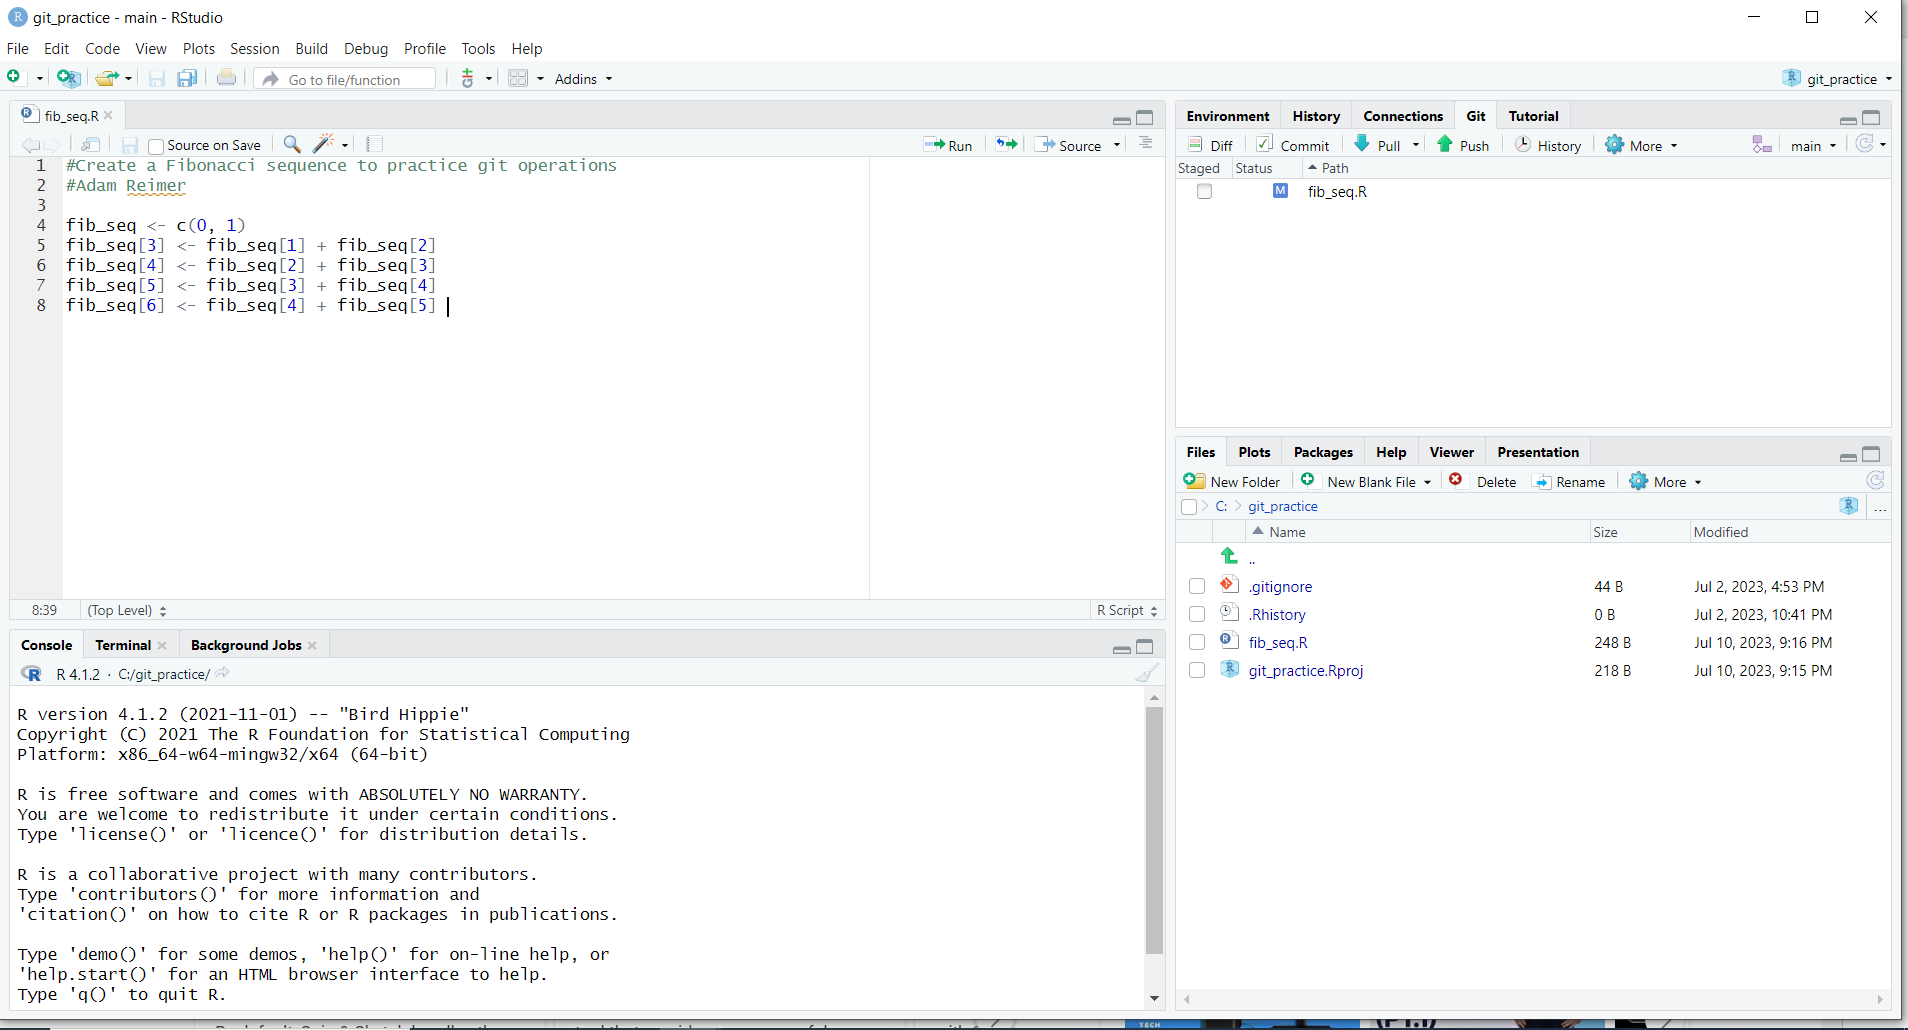
\includegraphics{RStudio_screen.PNG}

}

\caption{The RStudio windows with the Git pane shown in the top right
quadrant.}

\end{figure}

\hypertarget{git-init-1}{%
\subsection{git init}\label{git-init-1}}

If you are starting a brand new analysis creating a git repository at
the same time you create your R studio project is easy: \emph{New
Project\textgreater New Directory\textgreater New
Project\textgreater(provide name, location and check `create git
repository')}. This sequence runs git init in the background while the
RStudio project is created

\hypertarget{commands-accessible-through-the-git-tab}{%
\subsection{Commands accessible through the Git
tab}\label{commands-accessible-through-the-git-tab}}

\begin{itemize}
\item
  \texttt{git\ add} - add/Stage files by clicking the radio button next
  to each file in the RStudio Git pane.
\item
  \texttt{git\ diff}- the \emph{Diff} button will lead to another screen
  where the GUI allows users to \texttt{commit}, \texttt{diff} and
  \texttt{log} the repository.
\item
  \texttt{git\ commit} - the \emph{Commit} button will lead to another
  screen where the GUI allows users to \texttt{commit}, \texttt{diff}
  and \texttt{log} the repository.
\item
  \texttt{git\ pull} - the \emph{Pull} button allows the user to pull
  commits from the remote repository to the local repository.
\item
  \texttt{git\ push} - the \emph{Push} button allows the user to push
  commits from the local repository to the remote repository.
\item
  \texttt{git\ log} - the \emph{History} button will lead to another
  screen where the GUI allows users to \texttt{commit}, \texttt{diff}
  and \texttt{log} the repository.
\item
  \texttt{git\ revert} - the \emph{More} button will allow the user to
  \texttt{revert} a commit. IT also allows the user to add files to the
  \texttt{.gitignore} file by clicking the radio button next to the
  files you wish to ignore.
\item
  \texttt{git\ checkout\ -b} and \texttt{git\ remote} - the flowchart
  shaped button will allow you to create a new branch and add a remote
  to the repository.
\item
  \texttt{git\ checkout\ \textless{}new\_branch\textgreater{}} - the
  drop down list next to the word ``main'' will allow you to switch
  between branches.
\item
  Note the RStudio GUI is frequently slow to react to changes. The
  circular arrow refreshes the GUI. Often it will look like nothing is
  happening when you are clicking the radio buttons to add/stage files
  but clicking the refresh button will reveal the buttons were checked.
\end{itemize}

\begin{figure}

{\centering \includegraphics{Rstudio_Git.PNG}

}

\caption{The RStudio Git tab}

\end{figure}

\hypertarget{commands-accessible-through-the-diffcommithistory-window}{%
\subsection{Commands accessible through the Diff/Commit/History
window}\label{commands-accessible-through-the-diffcommithistory-window}}

\begin{itemize}
\item
  \texttt{git\ diff} - the \emph{Changes} tab will show line by line
  changes associated with the files in the working directory relative to
  the most recent commit. Old lines are shown in red while new line are
  shown in green.
\item
  \texttt{git\ commit} - the \emph{Changes} tab includes a commit
  message window and a \emph{Commit} button allowing the user to commit
  all of the staged changes. The commit title goes on the first line of
  the message window, followed by a blank line. The third line and
  onward contain the commit description.
\item
  \texttt{git\ log} - the \emph{History} tab will show the list of prior
  commits and the line by line changes associated with each file
  included in each commit.
\end{itemize}

\begin{figure}

{\centering 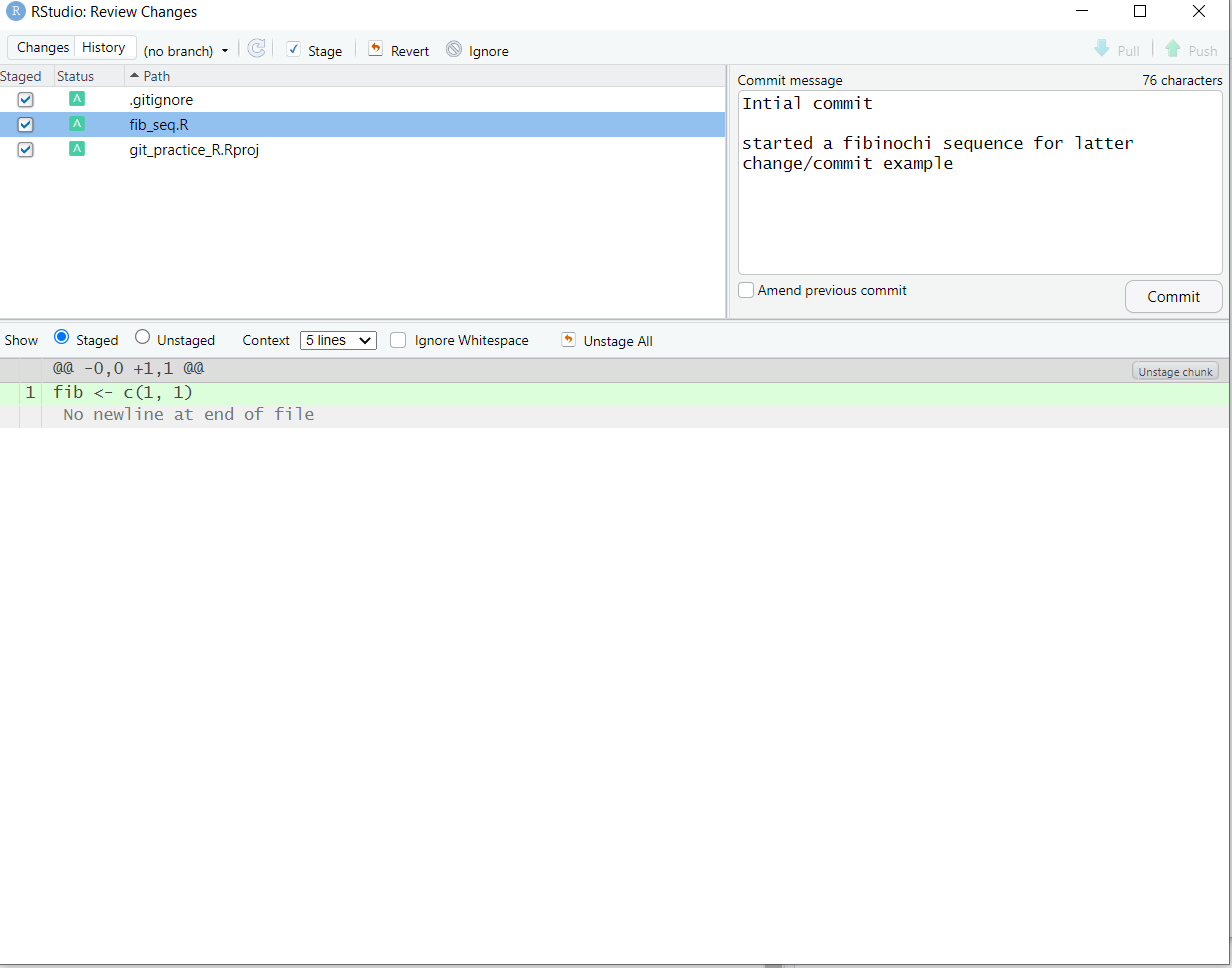
\includegraphics{Rstudio_commit.PNG}

}

\caption{The Diff/Commit/History window}

\end{figure}

\hypertarget{commands-not-accessible-using-the-rstudio-gui}{%
\subsection{Commands not accessible using the RStudio
GUI}\label{commands-not-accessible-using-the-rstudio-gui}}

To my knowledge you cannot use RStudio to:

\begin{itemize}
\item
  \texttt{git\ merge} two branches.

  \begin{itemize}
  \tightlist
  \item
    comment - This feels like a big deal if you intend to use Git
    optimally.
  \end{itemize}
\item
  \texttt{git\ checkout} to recall a single file from a previous commit.

  \begin{itemize}
  \tightlist
  \item
    comment - I've done this allot. It is sometimes possible to
    cut/paste a peice for revised code from the GUI history but it is
    usually formatted poorly which can be a pain if the section you need
    is large.
  \end{itemize}
\item
  \texttt{git\ checkout} to recall a prior commit to your working
  directory.

  \begin{itemize}
  \tightlist
  \item
    comment - Not needed often. I've generally been more interested in a
    single file.
  \end{itemize}
\item
  \texttt{git\ reset} to delete a local commit.

  \begin{itemize}
  \tightlist
  \item
    comment - I have done this rarely.
  \end{itemize}
\item
  Impress your friends by making your computer do things without using
  your mouse.

  \begin{itemize}
  \tightlist
  \item
    comment - My friends think I'm a dork and this only exacerbates
    things in that regard.
  \end{itemize}
\end{itemize}



\end{document}
